\documentclass{beamer}

\usepackage{tikz}
\usetikzlibrary{fit}
\usepackage{color}
\usepackage{booktabs}
\usepackage{tipa}
\usepackage{amssymb}
\usepackage{verbatim}
\usepackage[absolute,overlay]{textpos}
\usepackage{pifont}% http://ctan.org/pkg/pifont
\newcommand{\cmark}{\ding{51}}%
\newcommand{\xmark}{\ding{55}}%
\usetikzlibrary{bayesnet}
\usetikzlibrary{decorations.markings}


\newcommand{\nextForm}[1]{\rotatebox[origin=c]{270}{$_{\curvearrowright}$}$_{#1}$}

\title{Inducing Phonological Rules: Perspectives from Bayesian Program Learning}
\author{Kevin Ellis and Timothy O'Donnell and Joshua B. Tenenbaum and Armando Solar-Lezama}
\institute{MIT}
\date{2017}


\begin{document}

\frame{\titlepage}
%% \begin{frame}{Abstract}
%%     How do linguists come up with phonological rules? How do kids
%%     learn pig latin?  We develop computational models of these and
%%     other phenomena in language.  The unifying element of the models
%%     is to treat grammars as programs, which lets us apply ideas from
%%     the field of program synthesis to learn grammars. This lets the
%%     models capture phonological phenomena like vowel harmony or stress
%%     patterns and learn synthetic grammars used in prior studies of
%%     rule learning.  Going beyond individual grammar learning problems,
%%     we consider the problem of jointly inferring many related rule
%%     systems. By solving many textbook phonology problems, we can
%%     ask the model what kind of inductive bias best explains the
%%     attested phenomena.
%% \end{frame}




\begin{frame}{A language learning experiment}
  %  \fontsize{20}{7.2}\selectfont
  \Huge
  \centering\begin{tabular}{ll}
    \textipa{xau}&\visible<2->{\textipa{xauxaud@}}\\
    \textipa{man}&\visible<2->{\textipa{manmand@}}\\
    \textipa{kwaj}&\visible<2->{\textipa{kwajkwajd@}}\\
    \textipa{\c{c}in}&    \visible<2->{\textipa{\c{c}in\c{c}ind@}}\\
    \visible<3->{\textipa{lej}}&\visible<4->{\textipa{lejlejd@}}

  \end{tabular}
  \\\vspace{1cm}

  \visible<5->{\color{red}\texttt{A}$\to$\texttt{AA}$+$\textipa{d@}}

\end{frame}

\begin{frame}[t]{A language learning experiment}
  \begin{columns}

    \begin{column}{0.4\textwidth}
      
  \begin{center}
    \huge
    \begin{tabular}{ll}
      \textipa{dom} & \visible<2->{\textipa{domi}}\\
      \textipa{kot} & \visible<2->{\textipa{koti}}\\
      \textipa{lut} & \visible<2->{\textipa{lodi}}\\
      \textipa{vus} & \visible<2->{\textipa{vozi}}\\
      \textipa{wuk} & \visible<2->{\textipa{wugi}}\\
      \textipa{bur} & \visible<2->{\textipa{bori}}\\
      \visible<4->{\textipa{ruk}} & \visible<3->{\textipa{rogi}}\\
    \end{tabular}
  \end{center}
    \end{column}
        \begin{column}{0.6\textwidth}
        \visible<5->{\color{red}\Large  \texttt{A}$\to$\texttt{A}$ + /\text{i}/$
  
  \textipa{o}$\to$\textipa{u}$/$ \_ [-nasal +voice]\#

  [-sonorant]$\to$[-voice] $/$ \_ \#
  }
    \end{column}
    \end{columns}




\end{frame}

%% \begin{frame}{Learning to build and pronounce words}
%%   dog: [\textipa{dag}]\\
%%   dogs: [\textipa{dagz}]

%%   \vspace{1cm}\pause

%%   cat: [\textipa{k\ae t}]\\
%%   cats: [\textipa{k\ae ts}]\\

%%   \vspace{1cm}\pause

%%   /\textipa{dag}/+/\textipa{z}/ $\to$ /\textipa{dagz}/  $\to$  [\textipa{dagz}]

%%   /\textipa{k\ae t}/+/\textipa{z}/ $\to$ /\textipa{k\ae tz}/  $\to$  [\textipa{k\ae ts}]

%%   \vspace{0.5cm}

%%   z$\to$s / [-voice] \_ \#
  
%% \end{frame}

\begin{frame}{ABA (same/different/same)}
\centering\Huge  \begin{tabular}{l}
    wofewo\\
    lovilo\\
    fimufi
  \end{tabular}

  \pause

\vspace{1cm}  $\varnothing\to\sigma_i$ / $\sigma_i\sigma$ \_
  


  \vspace{1cm}

  /wofe/ $\to$ [wofewo]

\end{frame}

%% \begin{frame}{Three kinds of language learning}

%%   Child language acquisition

%%   \pause

%% \vspace{1cm}  Linguists discovering grammars

%%   \pause

%% \vspace{1cm}  Linguistics students doing problem sets

%% \end{frame}

%% \begin{frame}{Pig Latin}
%%   \begin{tabular}{l}
%%     \textipa{pIg}$\to$\textipa{Igpe}\\
%%     \textipa{latIn}$\to$\textipa{atIle}\\
%%     \textipa{\ae sk}$\to$\textipa{\ae ske}\\
%%   \end{tabular}

%%   \pause\vspace{1cm}

%%   \#$\to$[ ]$_i$ / \# [ -vowel ]$_i$ [ ]* \_
  
%%   \#$\to$e / \_

  
%% [ -vowel ]$\to\varnothing$ / \# \_ 
%% \end{frame}

\begin{frame}{Motivation}
  \Large \textbf{Problem:} Understand the principles that underlie linguistic generalization.\\\vspace{1cm} \textbf{Approach:} Triangulate these inductive principles with a wide variety of problems/data sets
\end{frame}

\begin{frame}{A (reverse) engineering problem}
  \Huge How is it possible 
  to learn a large number of diverse natural and artificial grammars from 
  relatively small data sets?
\end{frame}

\begin{frame}[t]{Bayesian Program Learning (BPL)}
\begin{textblock*}{5cm}(0cm,1cm)
\visible<2->{      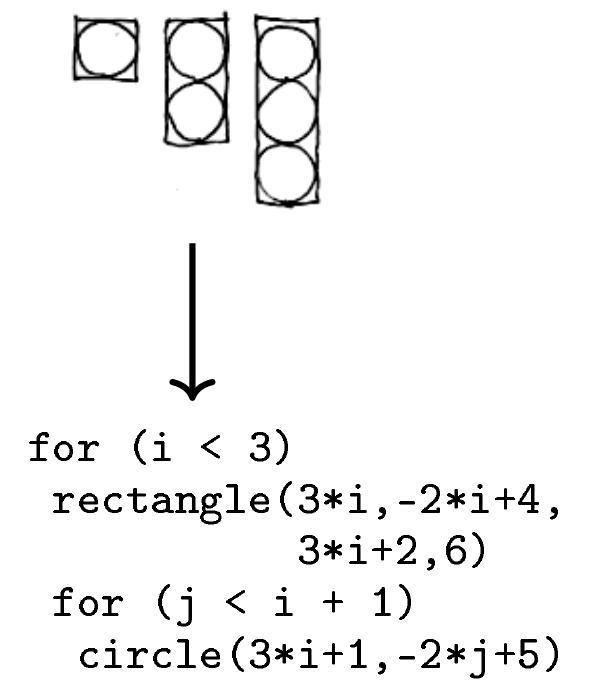
\includegraphics[width=4cm]{BPL1.png}}    \end{textblock*}
\begin{textblock*}{6cm}(0cm,6cm)
\visible<3->{      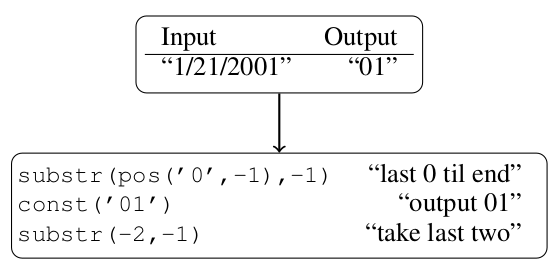
\includegraphics[width=6cm]{bpl2.png}}    \end{textblock*}
\begin{textblock*}{6cm}(6.5cm,2cm)
\visible<4->{      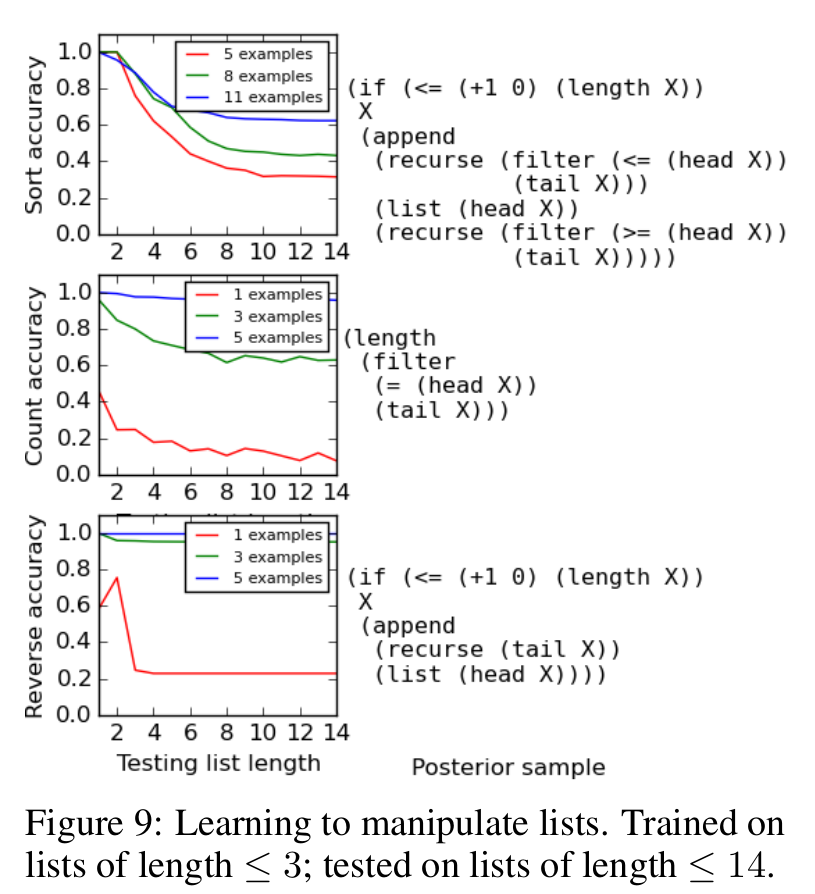
\includegraphics[width=6cm]{bpl3.png}}    \end{textblock*}
\end{frame}

\begin{frame}{Talk roadmap}

  \begin{itemize}
  \item Bayesian   program learning (BPL) for phonology
  \item Artificial grammar learning: using BPL as a tool for studying simplicity trade-offs
  \item Phonological rules in natural language: BPL as a tool for explaining a breadth of phenomena
  \item Simplicity metrics and universal grammar
  \item A problem with minimum description length as a simplicity metric
    \end{itemize}

  \end{frame}

\begin{frame}{Bayesian Program Learning (BPL) for phonology}
  %\hspace{-2cm}
  %\vspace{-4cm}
  \begin{textblock*}{5cm}(0cm,-3cm)
  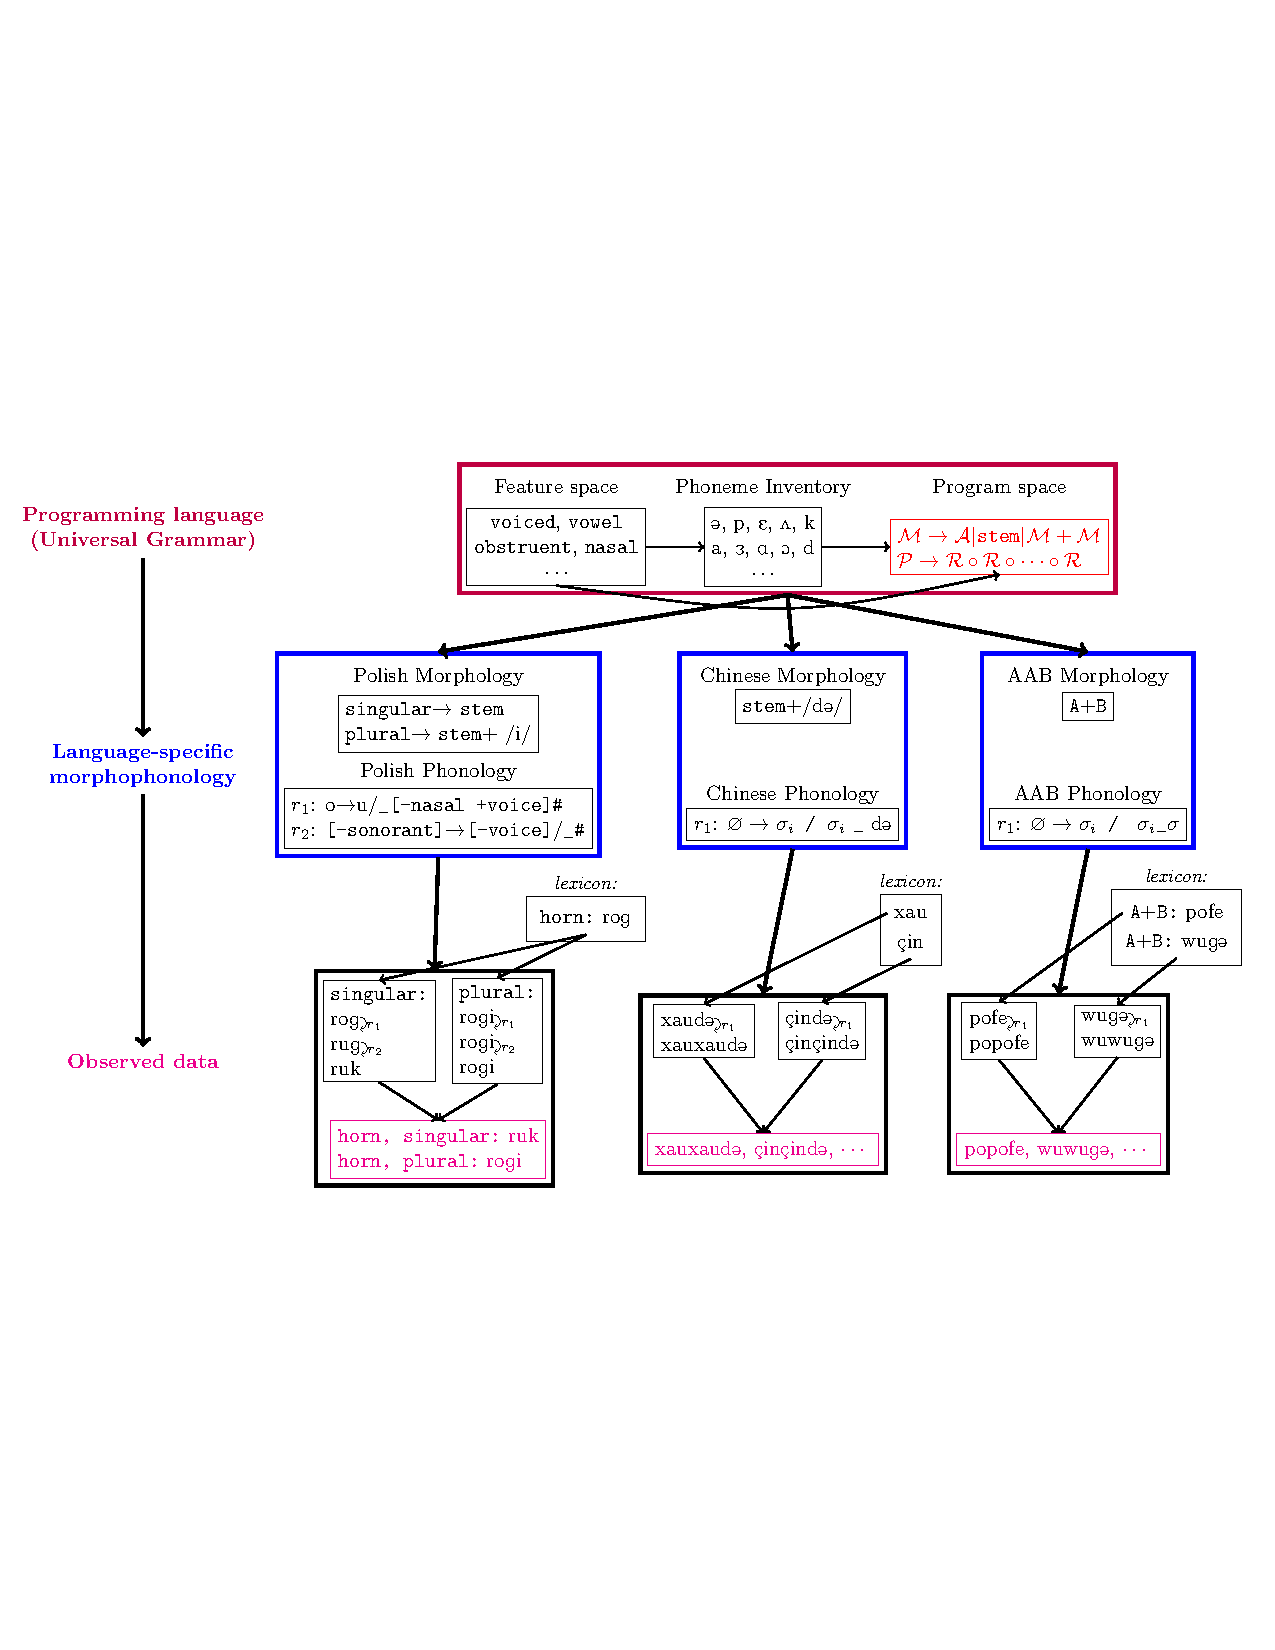
\includegraphics[pages={1}, width=12cm]{generativeModel.pdf}    \end{textblock*}
\end{frame}

\begin{frame}{What makes a good model?}
  Probable$\iff$low description length$\iff$simple

  \begin{equation*}
    \text{descriptionLength}(randomEvent) = -\log\mathbb{P} [randomEvent]
  \end{equation*}

    \pause
  
  \begin{eqnarray*}
    \text{descriptionLength}(\text{model}; \text{data}) &=& \text{descriptionLength}(\text{model})\\& +& \sum_{x\in \text{data}}\text{descriptionLength}(x ; \text{model})
  \end{eqnarray*}

  \pause

  \begin{equation*}
    \text{descriptionLength}(\text{model}) \sim \text{program size}
  \end{equation*}

  \pause


  \begin{gather*}
    \text{descriptionLength}(x ; \text{model})  = \text{size of \emph{x}'s UR in model} \\
    \text{descriptionLength}(\text{[\textipa{pofepo}]}; \text{ABA}) = \text{len(/\textipa{pofe}/)} = 4\\
        \text{ (see Richard Futrell's talk)}
  \end{gather*}

  \pause

  \textbf{Bayesian Program Learning framed as compression}\\
  \textbf{Old idea from Solomonoff}
  
\end{frame}



\begin{frame}{The program space}
\begin{textblock*}{5cm}(0cm,-3cm)
  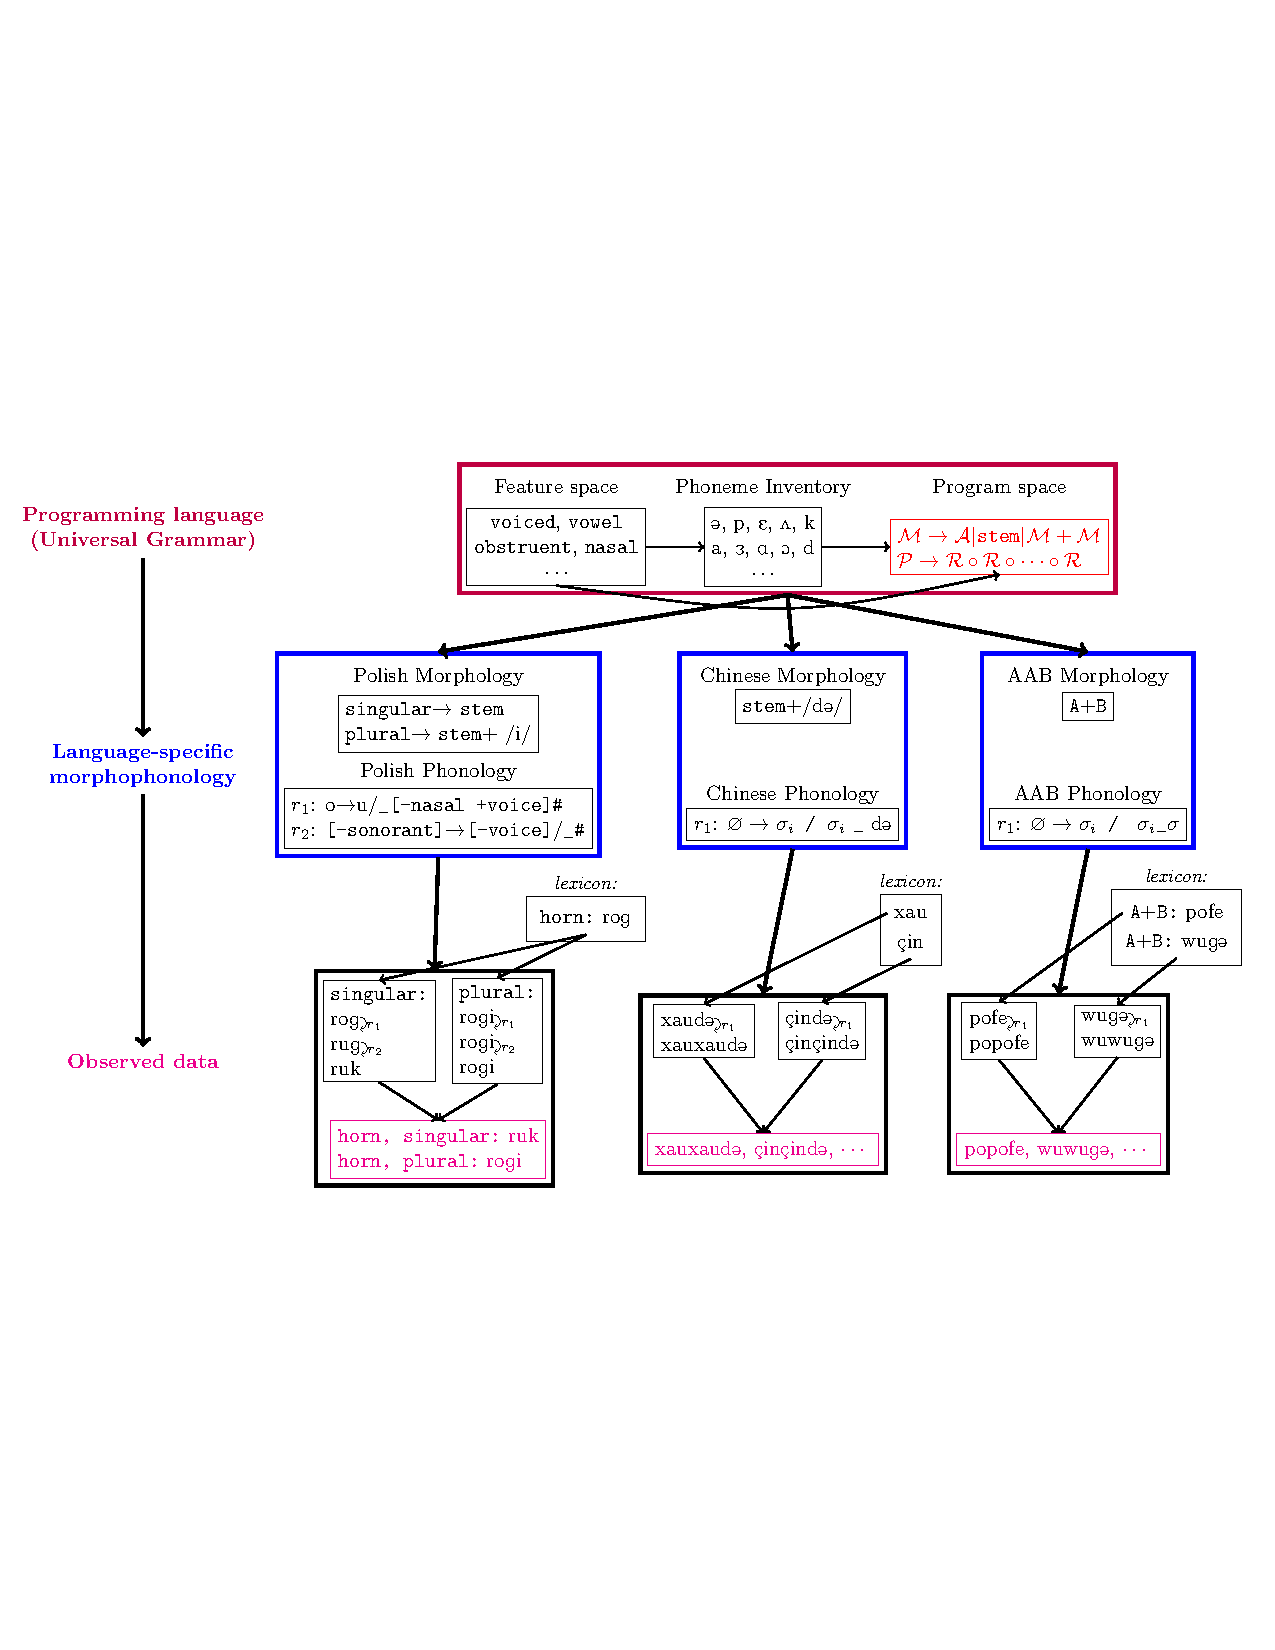
\includegraphics[pages={1}, width=12cm]{generativeModel.pdf}    \end{textblock*}
\begin{tikzpicture}[remember picture,overlay]
\draw[green, very thick] (6,2.5) ellipse (3cm and 1.5cm);
\end{tikzpicture}  
  \end{frame}
\begin{frame}{The program space: SPE-style context-sensitive rewrites}
  \begin{tabular*}{\textwidth}{ll}
\toprule
Grammar rule  & English description \\\midrule
$\mathcal{P}\to \mathcal{R}\circ \mathcal{R}\circ \cdots \circ \mathcal{R}$&\textbf{P}honology is compositions of \textbf{r}ewrites\\
$\mathcal{R}\to \mathcal{F}\longrightarrow \mathcal{C} / \mathcal{T}\_\mathcal{T}$& Rewrite \textbf{f}ocus to \textbf{c}hange between \textbf{t}riggers\\
$\mathcal{T}\to \# \mathcal{T}' | \mathcal{T}'$ & \textbf{T}riggers optionally match end of string, \#\\
$\mathcal{T}'\to \epsilon | \mathcal{X} \mathcal{T}' | \mathcal{X}^* \mathcal{T}'$ & \textbf{T}riggers are sequences of matrices $\mathcal{X}$\\
$\mathcal{X}\to a|t|s|\cdots$&Matrices can be constant phonemes\\
$\mathcal{X}\to [\pm \mathcal{E} \; \pm \mathcal{E} \; \cdots \; \pm \mathcal{E}]$& Matrices check features $\mathcal{E}$\\
$\mathcal{E}\to \text{voice}|\text{nasal}|\cdots$&Standard phonological f\textbf{e}atures\\
$\mathcal{F}\to \mathcal{X}$&Focus can be a feature matrix\\
$\mathcal{F}\to\mathbb{Z}$&Focus can be one of the triggers (copies it)\\
$\mathcal{F}\to\varnothing$&Insertion rule\\
$\mathcal{C}\to\mathcal{X}$&Structural change can be a feature matrix\\
$\mathcal{C}\to\varnothing$&Deletion rule\\
$\mathcal{C}\to\mathbb{Z}$&\begin{tabular}{l}
  Structural change constrained to\\ match a triggering feature matrix
  \end{tabular}
\bottomrule
\end{tabular*}

\end{frame}

\begin{frame}{The programs}
\begin{textblock*}{5cm}(0cm,-3cm)
  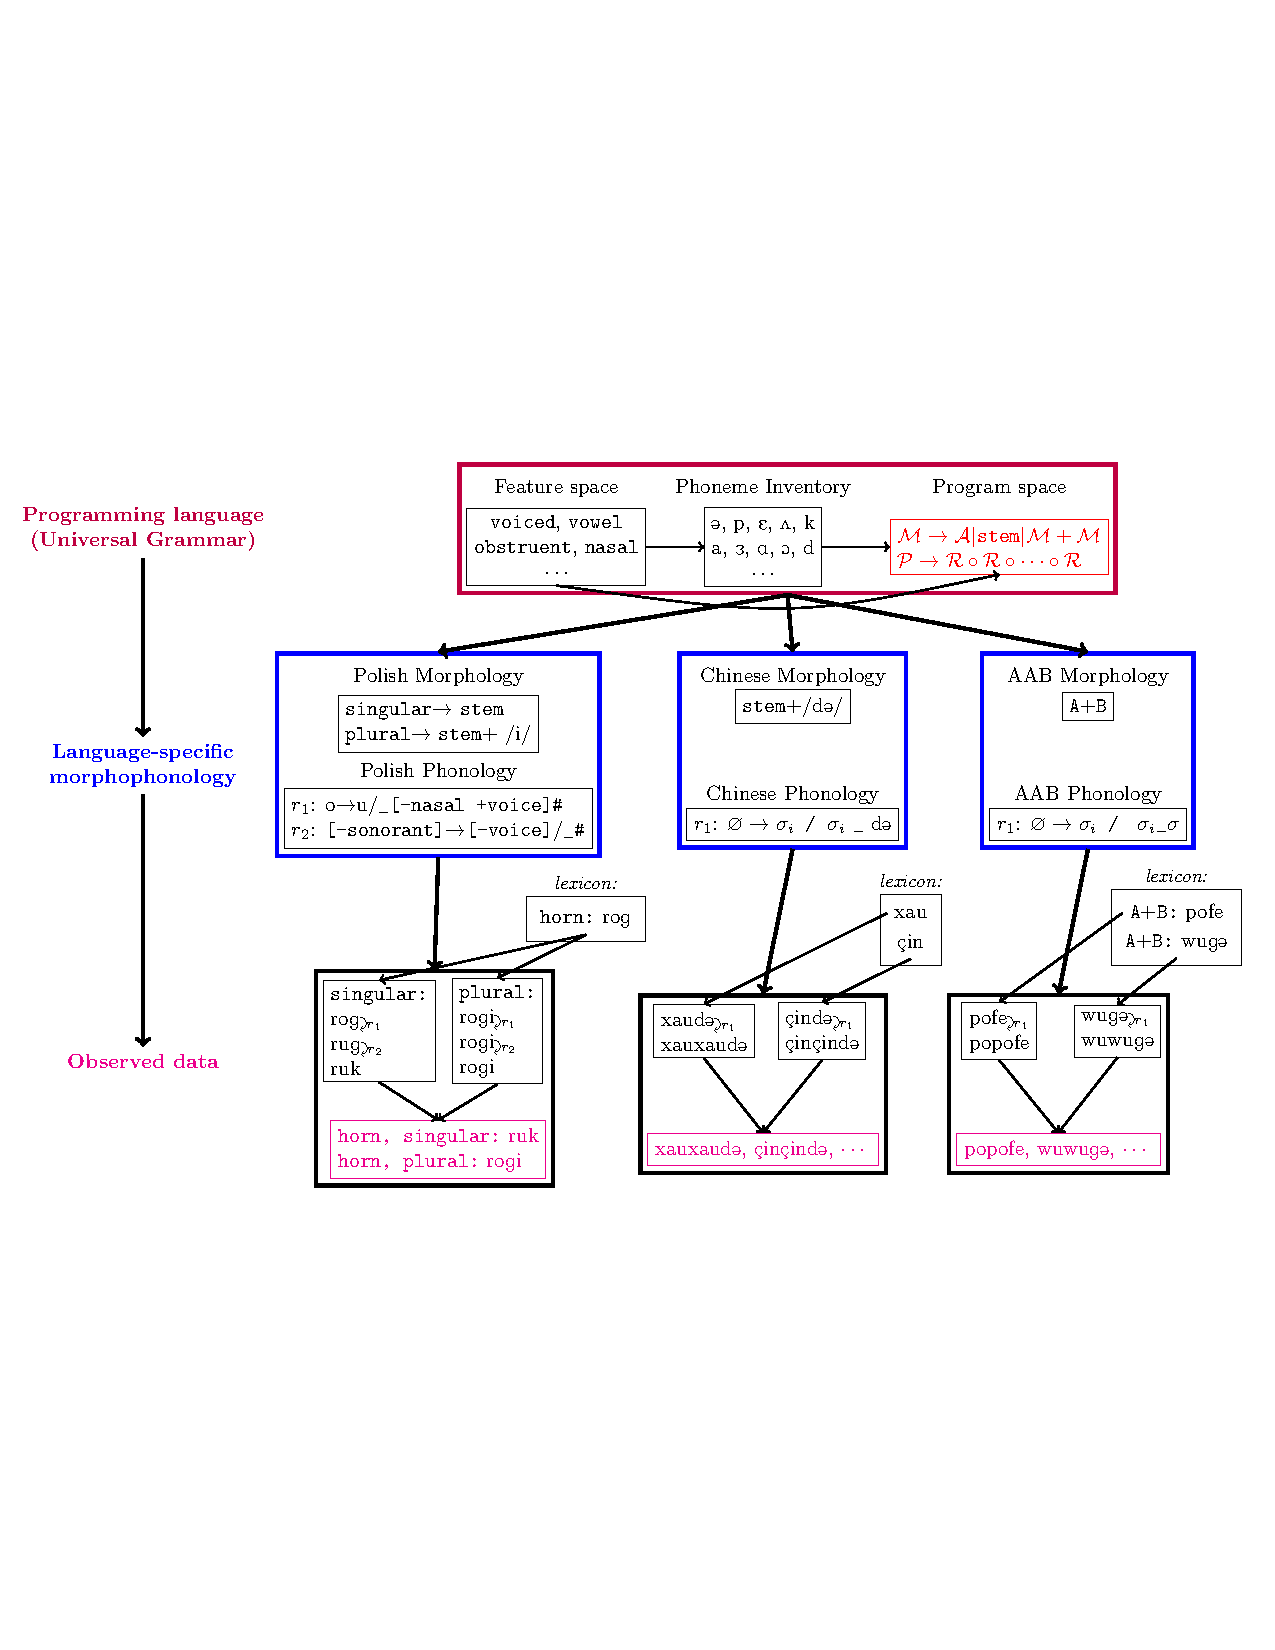
\includegraphics[pages={1}, width=12cm]{generativeModel.pdf}    \end{textblock*}
\begin{tikzpicture}[remember picture,overlay]
\draw[green, very thick] (3,0.25) ellipse (2cm and 1.5cm);
\end{tikzpicture}  
\end{frame}

\begin{frame}{The programs}
  \begin{itemize}
  \item Morphology: Simple concatenative rules combining
    underlying forms of morphemes based on
    morphological function.
  \end{itemize}
  SING: \# + rog + \#
  \\PLURAL: \# + rog + i + \#

  \begin{itemize}
  \item Phonology: Ordered rules that transform resulting phone sequences.
  \end{itemize}
  \textipa{o}$\to$\textipa{u}$/$ \_ [-nasal +voice]\#\\
  obstruent$\to$ [-voice] $/$\_\#
\end{frame}

\begin{frame}{The lexicon}
\begin{textblock*}{5cm}(0cm,-3cm)
  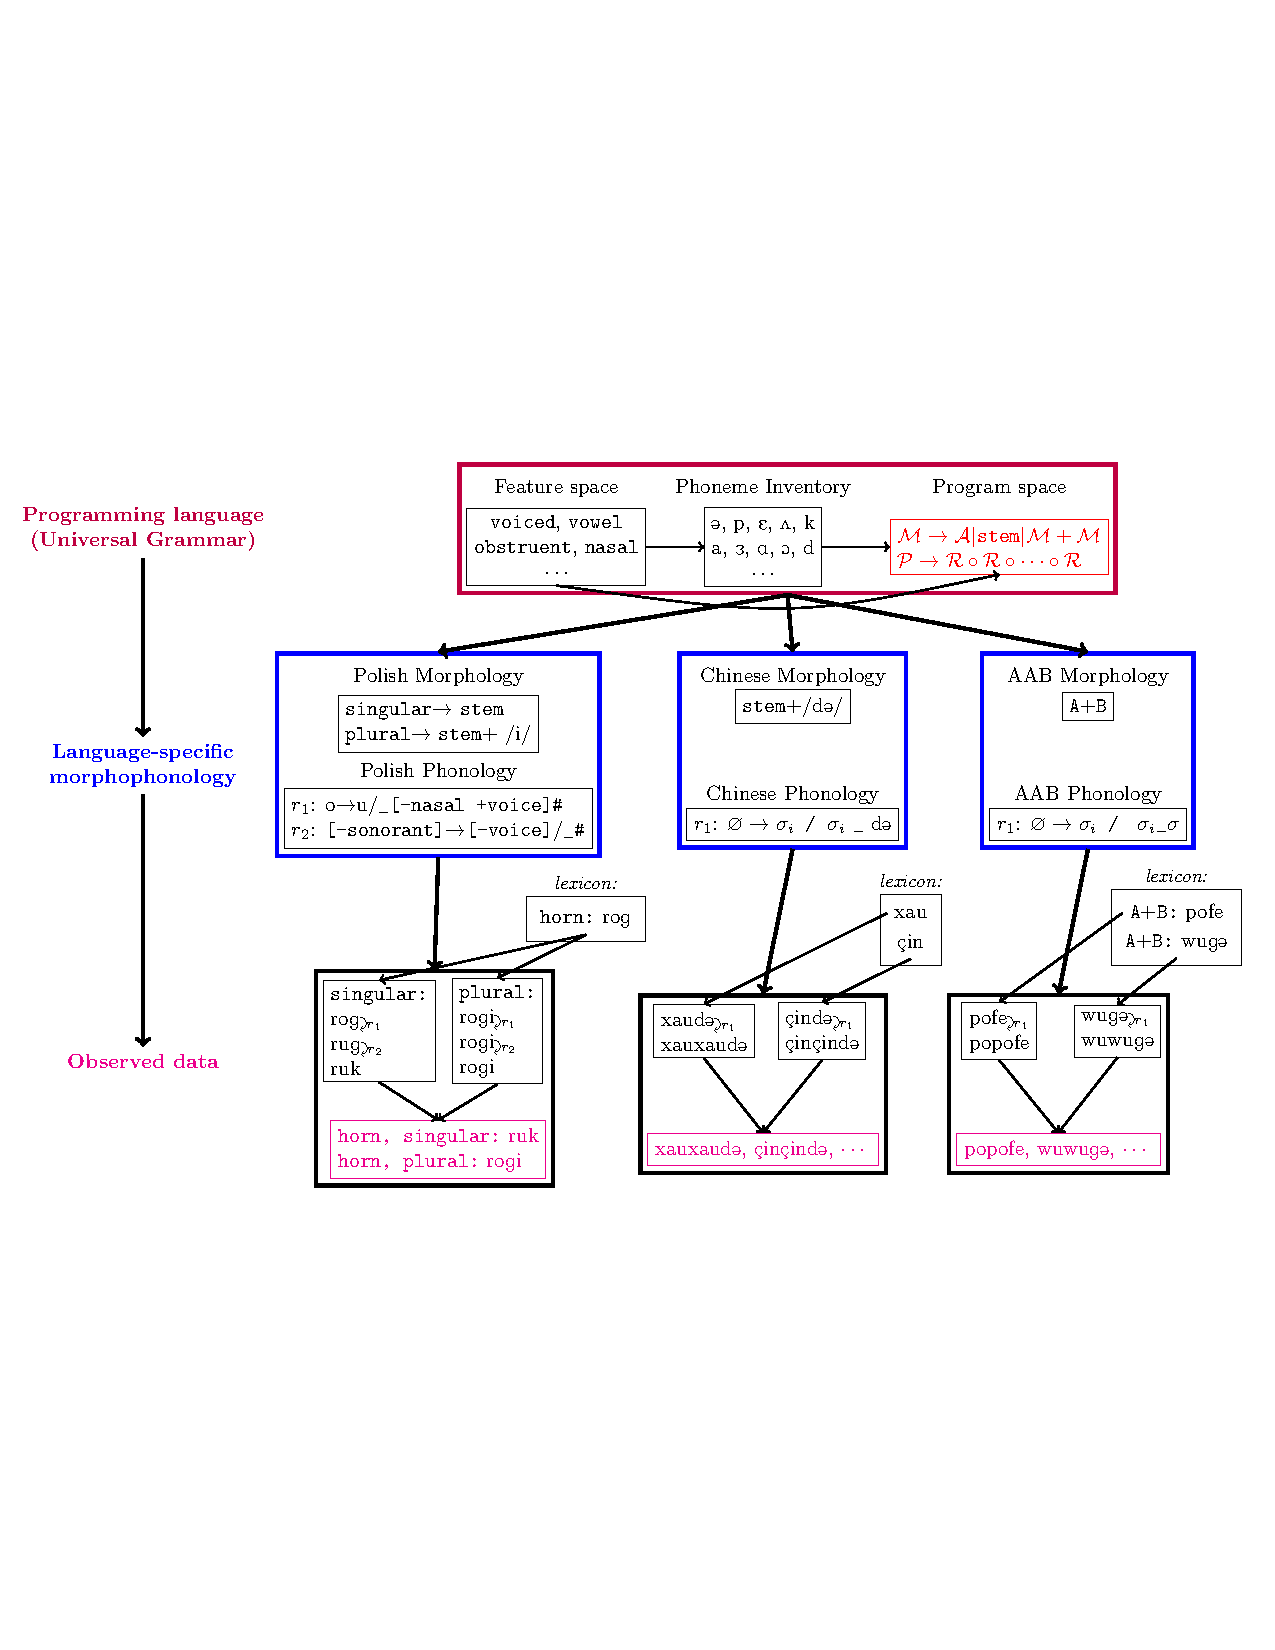
\includegraphics[pages={1}, width=12cm]{generativeModel.pdf}    \end{textblock*}
\begin{tikzpicture}[remember picture,overlay]
  \draw[green, very thick] (4.5,-1.5) ellipse (0.75cm and 0.75cm);
  \draw[green, very thick] (7.5,-1.5) ellipse (0.75cm and 0.75cm);
  \draw[green, very thick] (10,-1.5) ellipse (0.75cm and 0.75cm);
\end{tikzpicture}  
\end{frame}

\begin{frame}{The lexicon}
  \large
  
  Inventory of stems (``underlying representations'')

  
  \vspace{1cm}
  \centering
\begin{columns}[T] % align columns
  \begin{column}{.25\textwidth}
  \textbf{Polish}:    
  \\\begin{tabular}{l}
    
    rog\\
    klub\\
    dvon\\
    ...
    \end{tabular}

    \end{column}%
%\hfill%
\begin{column}{.25\textwidth}
\textbf{AAB:}
\\\begin{tabular}{l}
pofe\\
wuga\\
...
  \end{tabular}
  

  
      \end{column}%
\end{columns}

\vspace{1cm}

Shorter stem$\iff$Better compression$\iff$Higher likelihood of data 

\end{frame}



\begin{frame}{}

  \Huge
\centering  But how do you find any good programs in the first place?
  
  \end{frame}



\begin{frame}{The search problem}
  \textbf{program synthesis techniques from Armando Solar-Lezama}
  \begin{columns}[T] % align columns
    \begin{column}{.6\textwidth}
      \rule{\linewidth}{4pt}
      \emph{SAT/SMT solving:}
\centering  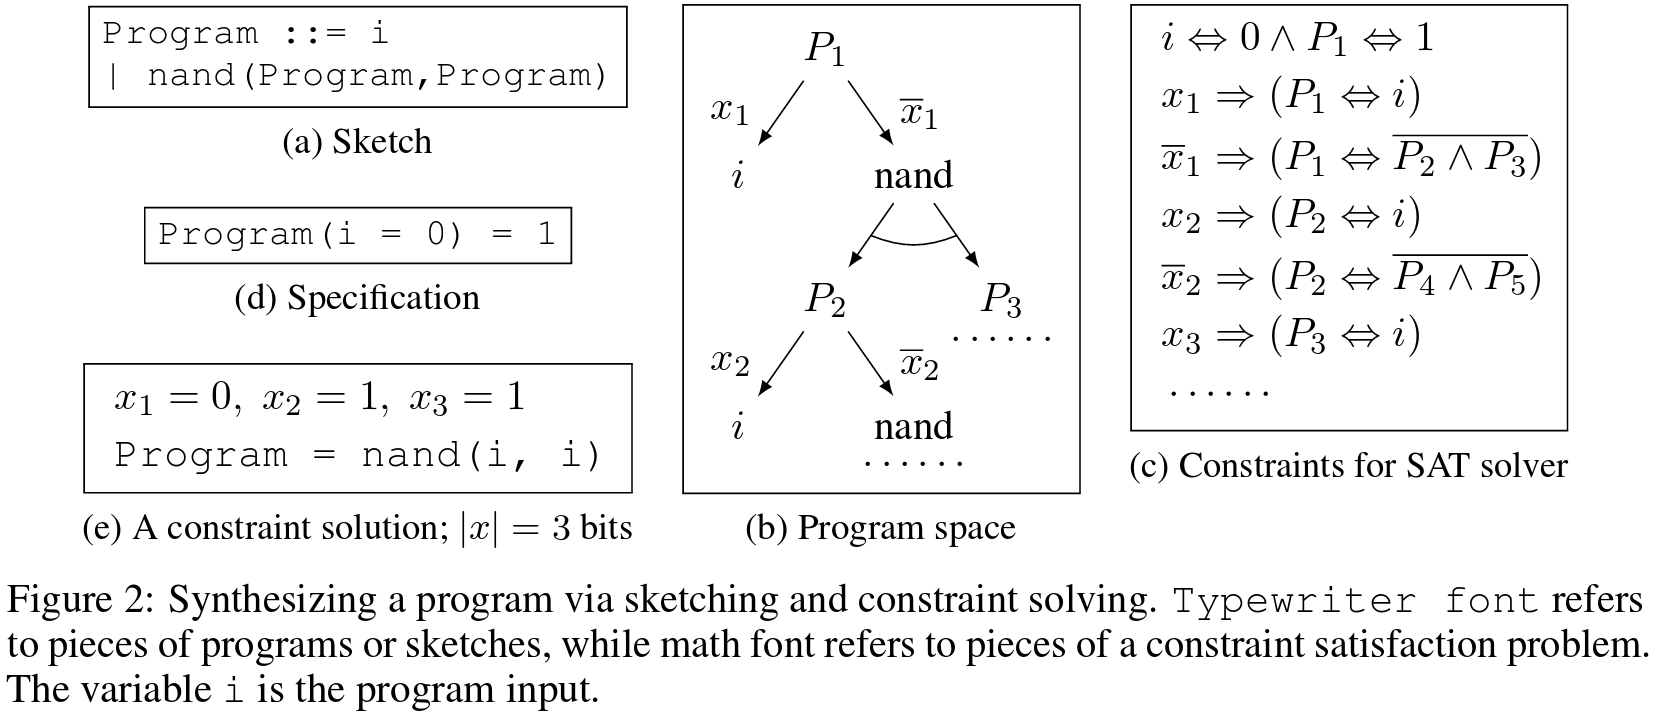
\includegraphics[width = 6cm]{background.png}
    \end{column}%
\hfill%
\begin{column}{.5\textwidth}
  \rule{\linewidth}{4pt}
  \emph{Sketch:}
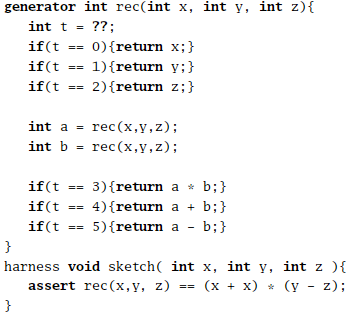
\includegraphics[width = 5cm]{generatorExample.png}
  

  
      \end{column}%
  \end{columns}
  \pause

  \Large
  \textcolor{green}{\cmark} Guarantee: Exact optimization
  \\  \textcolor{red}{\xmark} No guarantee: runtime
  \pause

  2 rules, 1 inflection: $\geq (10^{18}\text{rules})^2\times (10^{8} \text{morphologies}) = 10^{42}\text{models}$


\end{frame}



\begin{frame}{Artificial Grammar Learning}

  Widely studied. \\\\Fundamental hypothesis: AGL engages some shared resources with first language acquisition

  \\\\

  \begin{itemize}
  \item ABA (same/different/same): wofewo, \textipa{pik\ae pi}, gugagu
  \item ABB (different/same/same): wowofe, \textipa{pipik\ae}, guguga
  \item Pig Latin
    \item $\cdots$
    \end{itemize}

\end{frame}

\begin{frame}{Artificial Grammar Learning}

  \begin{centering}
   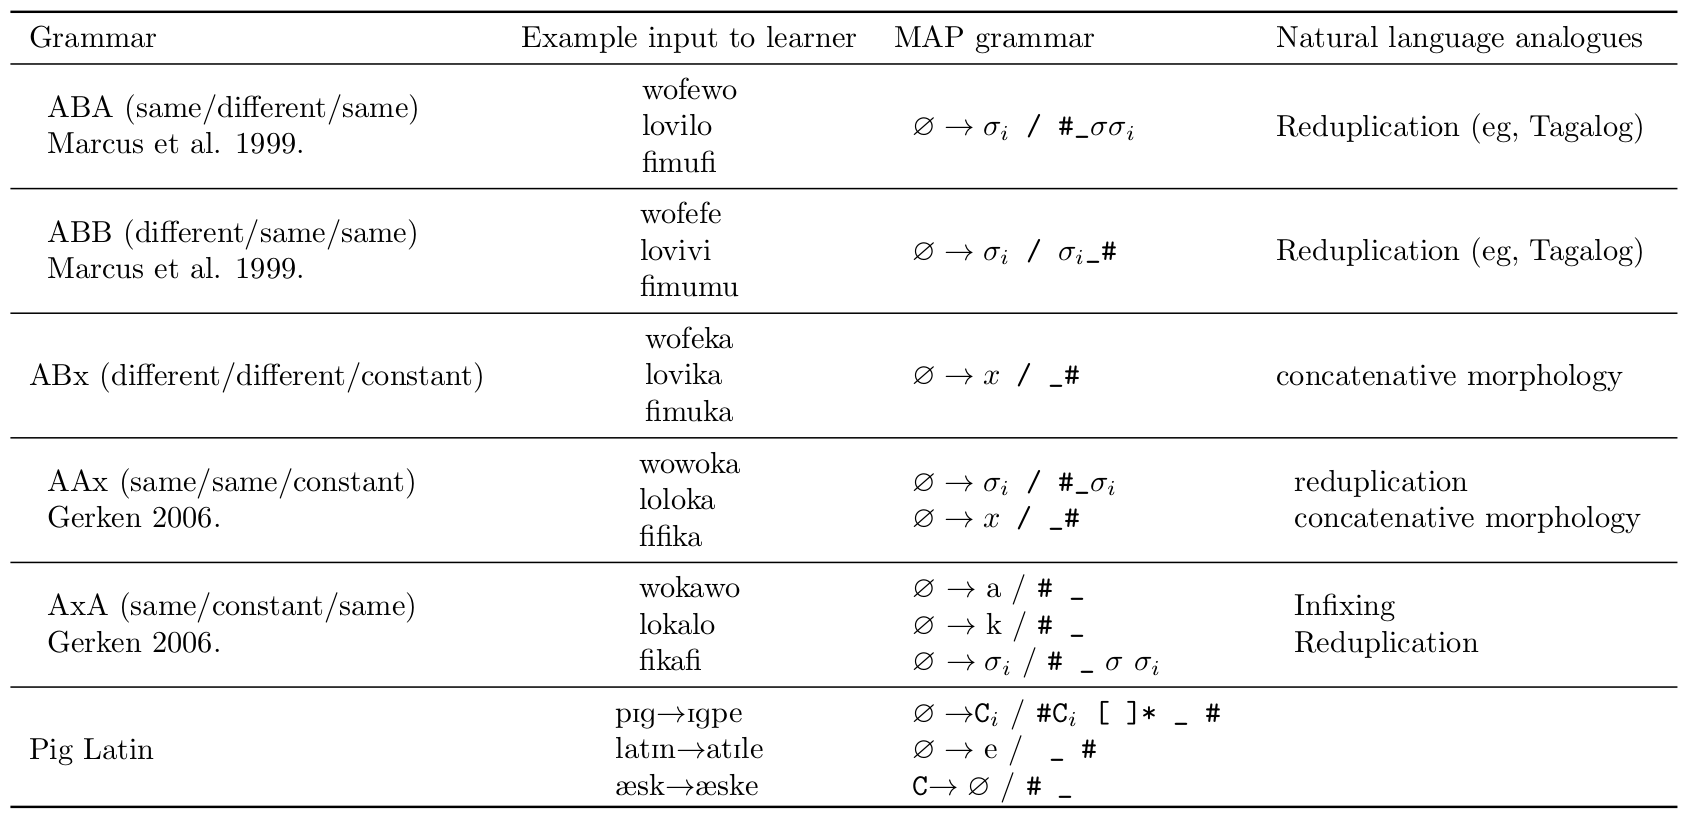
\includegraphics[width = 11.5cm]{synthetic.png}
  \end{centering}

  Marcus 1999: Babies learn these grammars\\
  Gerken 2006: Babies learn these grammars \emph{from only a few examples}\\

\end{frame}

\begin{frame}{Optimal simplicity front for learning ABB from  1 example}
  \centering  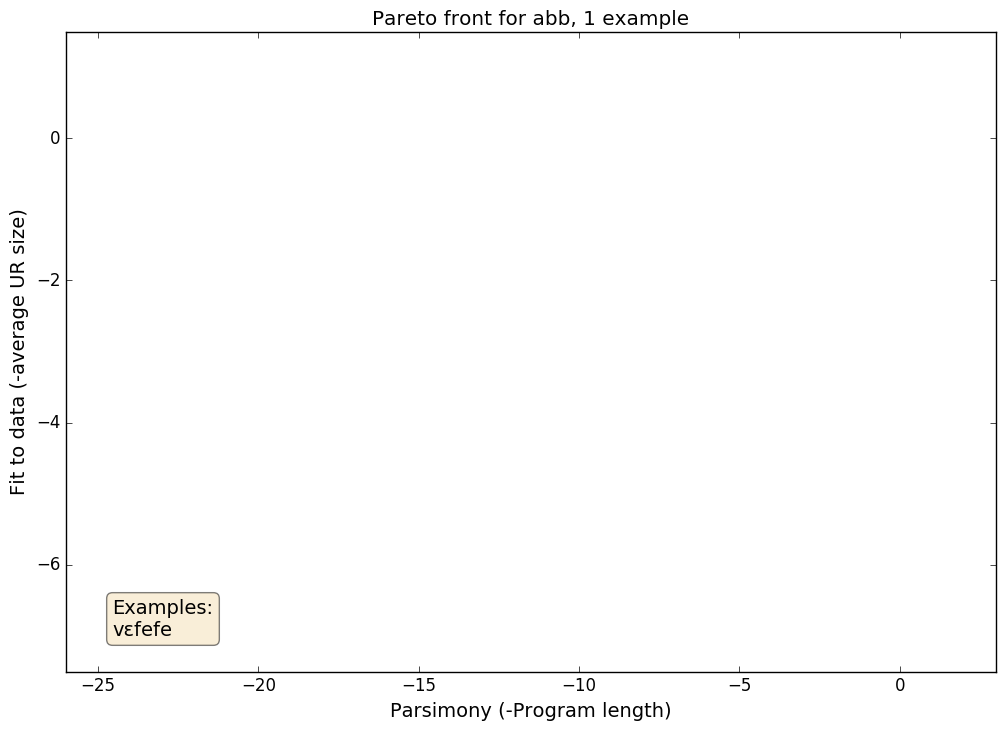
\includegraphics[width = 11cm]{marcusAnimation0.png}   
\end{frame}
\begin{frame}{Optimal simplicity front for learning ABB from  1 example}
  \centering  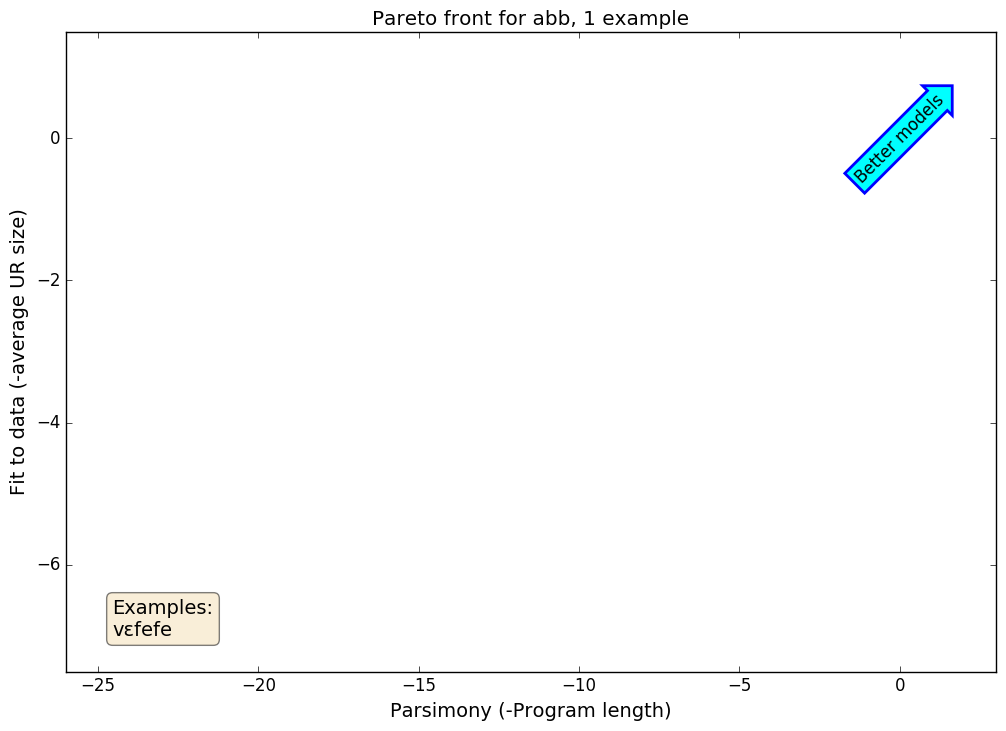
\includegraphics[width = 11cm]{marcusAnimation1.png}   
\end{frame}
\begin{frame}{Optimal simplicity front for learning ABB from  1 example}
  \centering  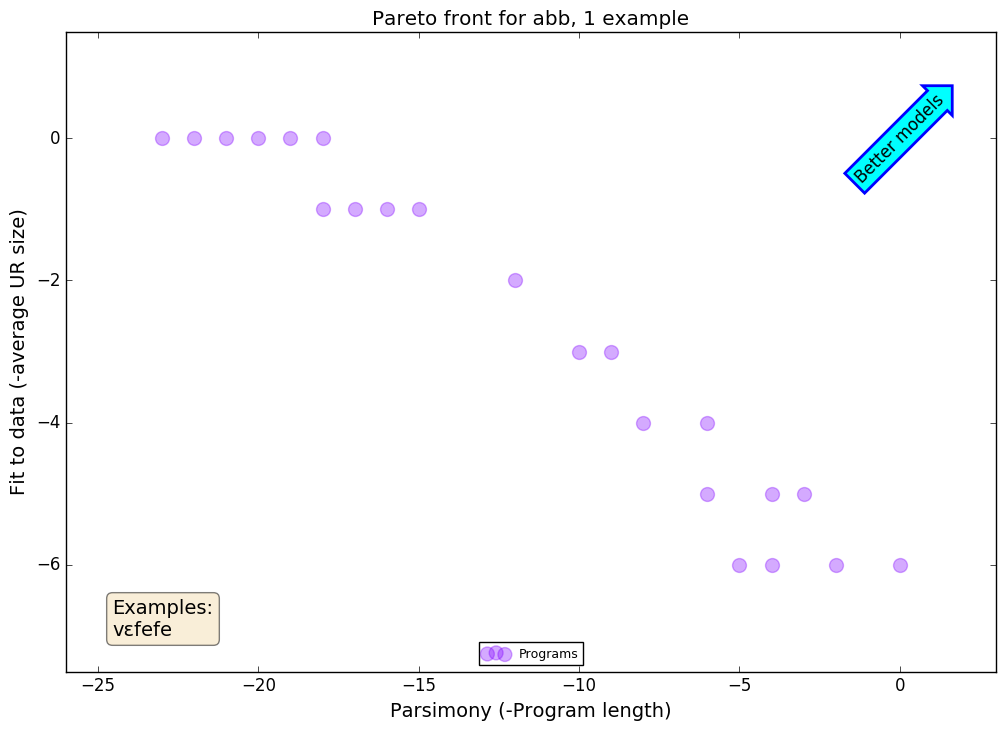
\includegraphics[width = 11cm]{marcusAnimation2.png}   
\end{frame}
\begin{frame}{Optimal simplicity front for learning ABB from  1 example}
  \centering  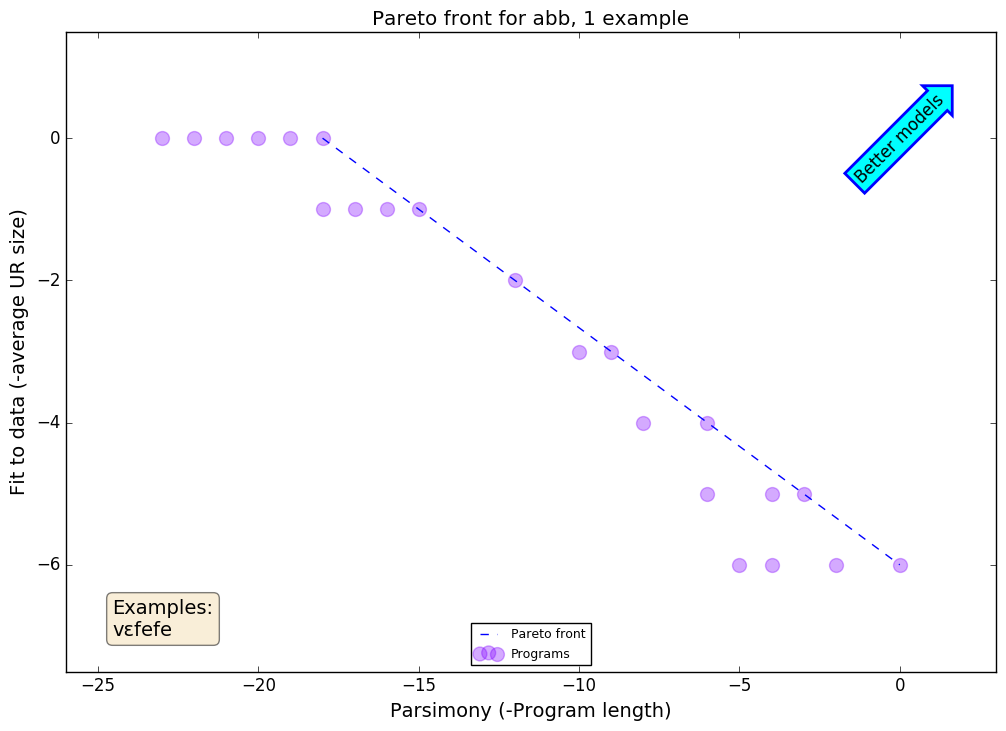
\includegraphics[width = 11cm]{marcusAnimation3.png}    
\end{frame}
\begin{frame}{Optimal simplicity front for learning ABB from  1 example}
  \centering  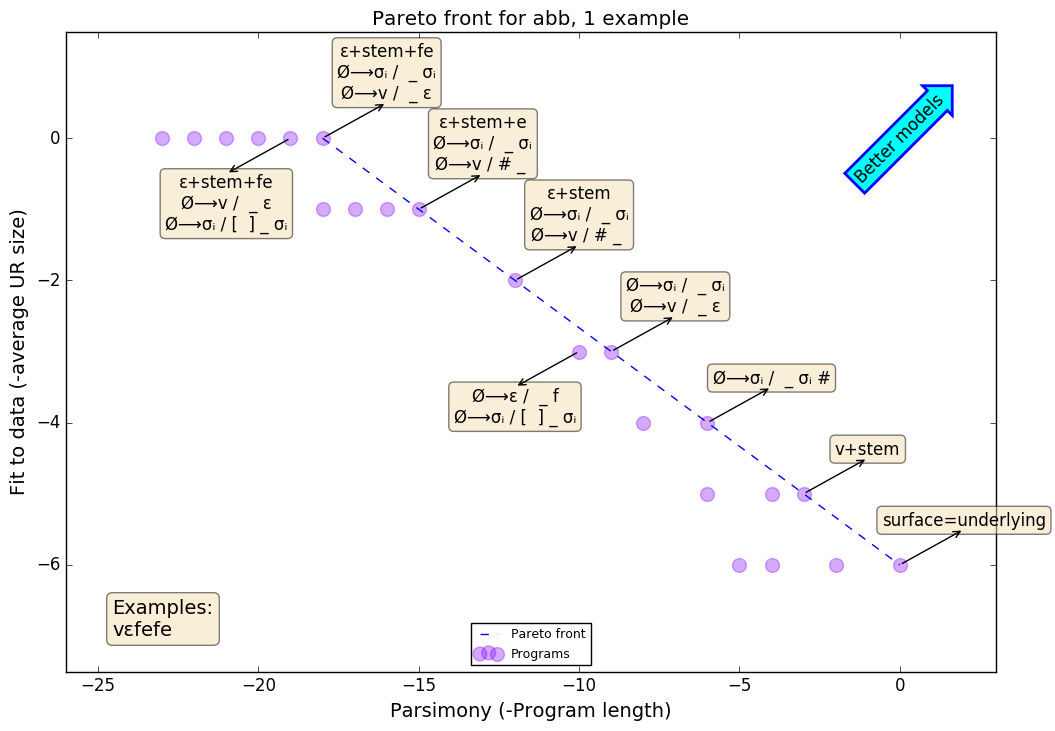
\includegraphics[width = 11cm]{marcusAnimation4.png}   
\end{frame}

\begin{frame}{Optimal simplicity front for learning ABB: 2 examples}
  \centering  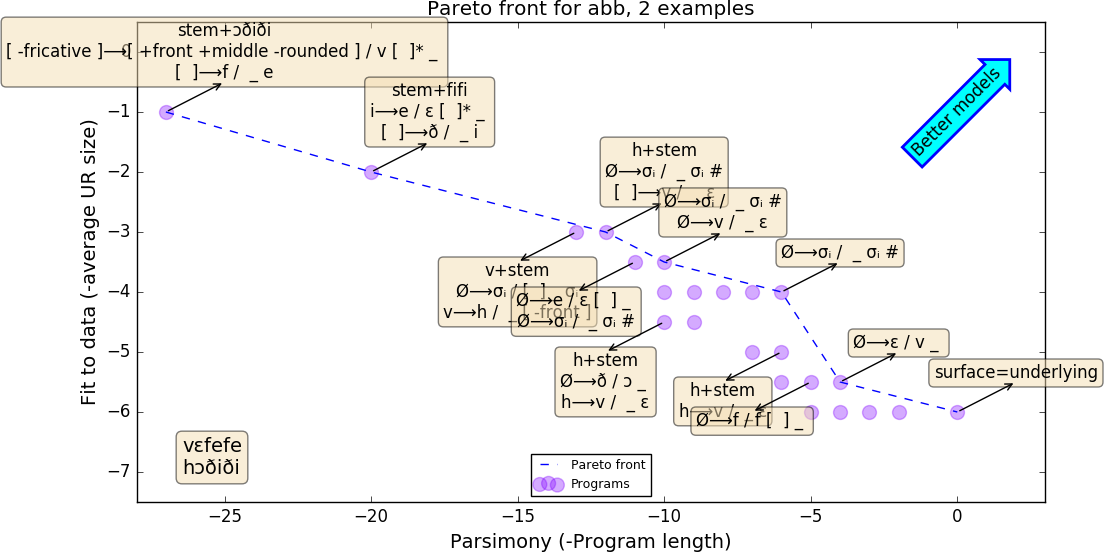
\includegraphics[width = 11cm]{syllableFront2.png}  
\end{frame}

\begin{frame}{Optimal simplicity front for learning ABB: 3 examples}
  \centering  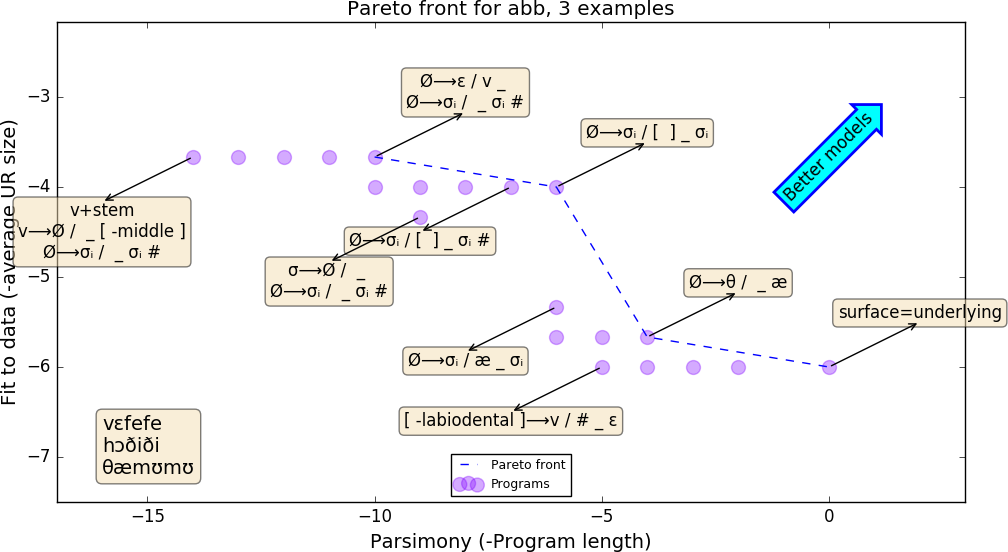
\includegraphics[width = 11cm]{syllableFront3.png}  
\end{frame}


%% \begin{frame}{Learning ABB: 5 examples}
%%   \centering  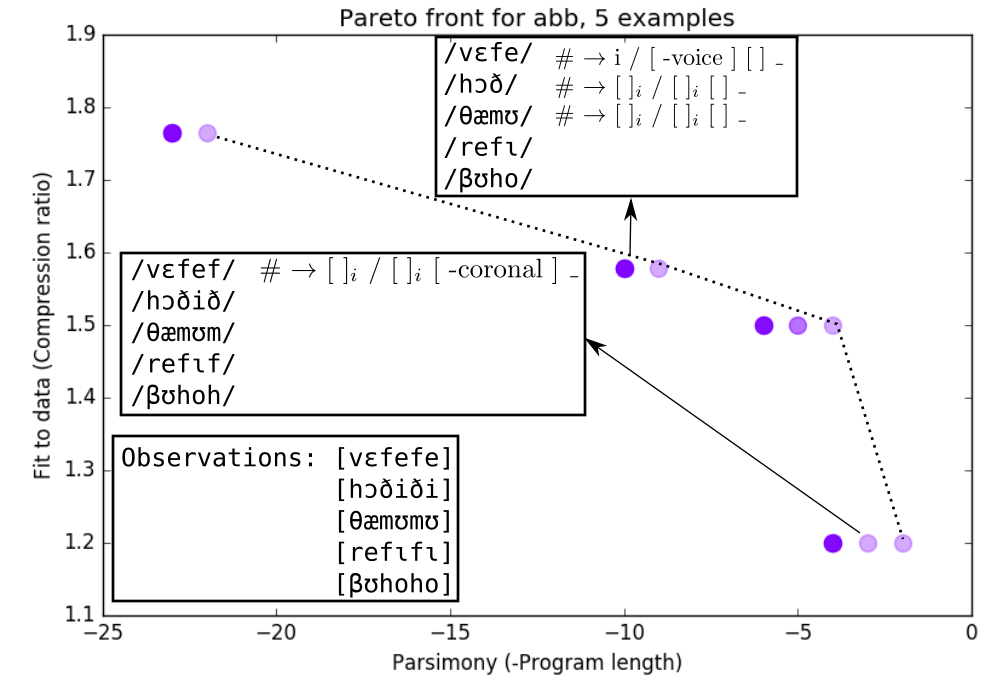
\includegraphics[width = 11cm]{front5.png}  
%% \end{frame}  safe compile latex

\begin{frame}{Optimal simplicity front for learning ABB without syllables, 3 examples}
    \centering  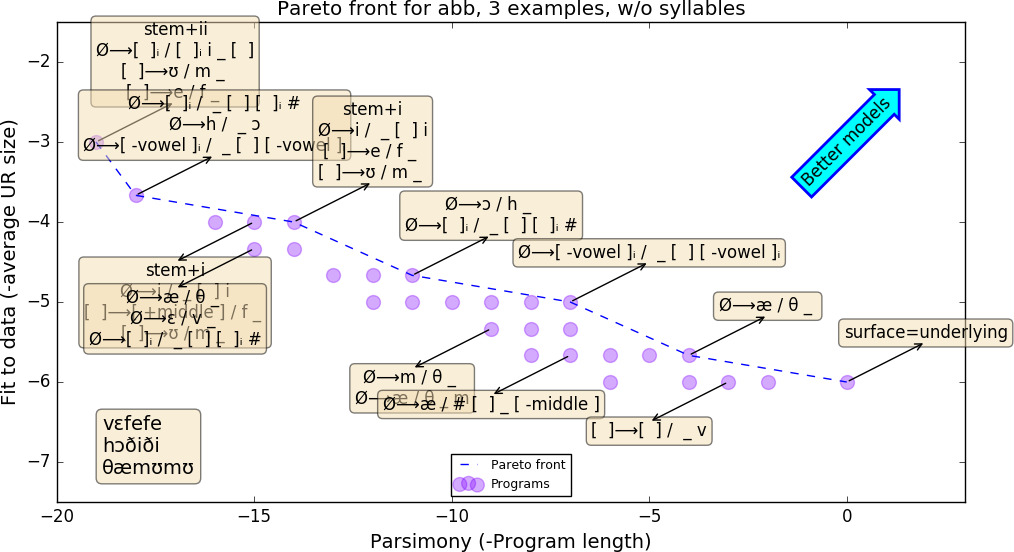
\includegraphics[width = 11cm]{front3.png}  
\end{frame}

\begin{frame}{Optimal simplicity front for learning ABB without syllables, 6 examples}
    \centering  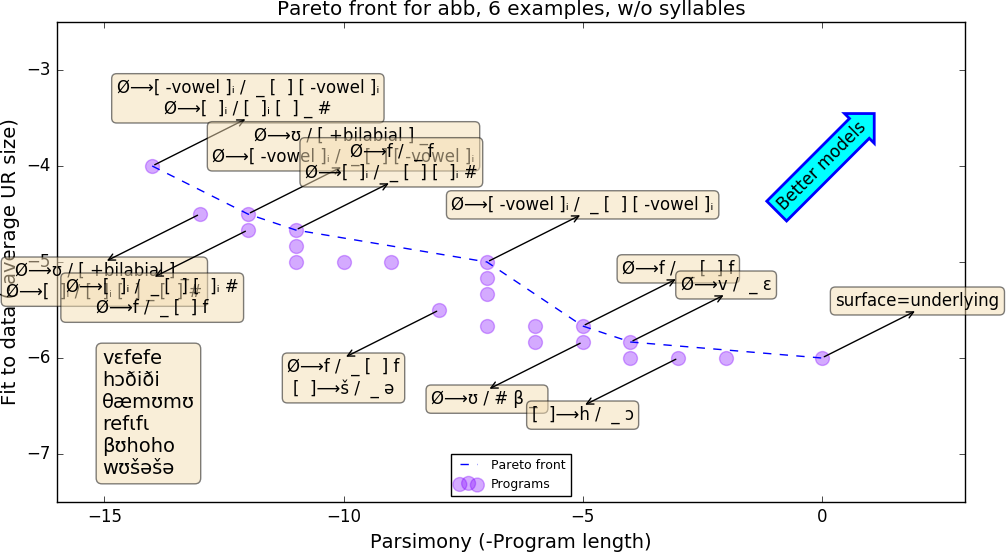
\includegraphics[width = 11cm]{front6.png}  
  \end{frame}

\begin{frame}{Learning natural language phonology}
  The vision: Induce programs describing diverse phonological systems from many languages. Imagine getting data from field linguists

  \vspace{1cm}
Ours is not the first linguistic rule learner: Ezer Rasin \&  Roni Katzir (this workshop); Albright \& Hayes 2003; Yip \& Sussman 1996; Constantine Lignos \& Charles Yang 2010; Doyle \& Bicknell \& Levy 2014; Colin Wilson 2006

\vspace{1cm}

\large \textbf{What is a good stepping stone toward this vision?}
  \end{frame}

\begin{frame}{Doing your phonology homework}

  \begin{textblock*}{10cm}(0.5cm,1.5cm)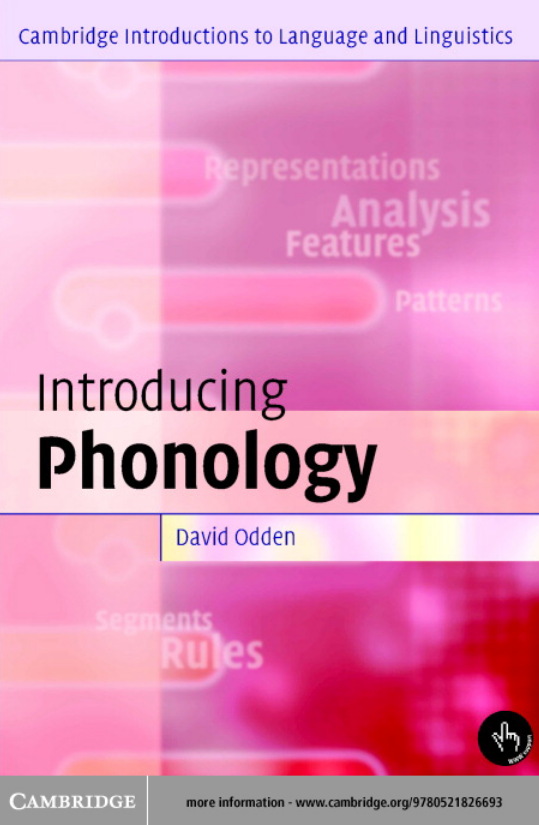
\includegraphics[width=5cm]{phonologyCover.png}\end{textblock*}

  \begin{textblock*}{10cm}(2.5cm,1.3cm)\visible<2>{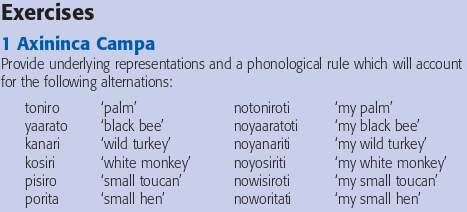
\includegraphics[width=10cm]{phonology1.png}}\end{textblock*}

  %    \begin{textblock*}{10cm}(2.5cm,1.3cm)\visible<3->{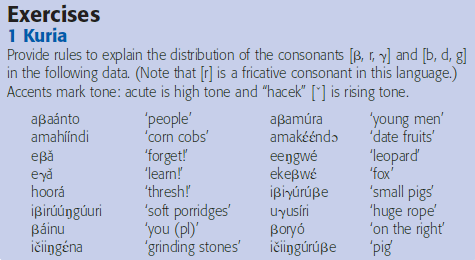
\includegraphics[width=10cm]{alternationExample.png}}\end{textblock*}
  \begin{textblock*}{10cm}(0.5cm,1.3cm)\visible<3->{\frame{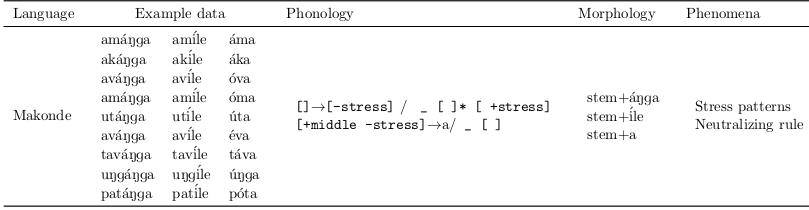
\includegraphics[width=12cm]{exampleProblem1.png}}}\end{textblock*}
  \begin{textblock*}{10cm}(1cm,2.3cm)\visible<4->{\frame{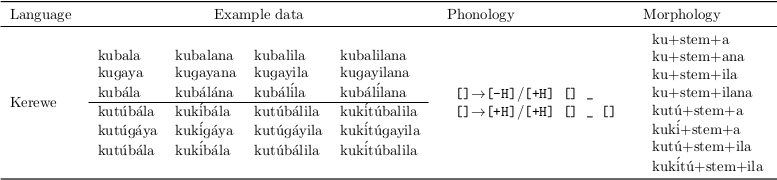
\includegraphics[width=12cm]{exampleProblem2.png}}}\end{textblock*}
  \begin{textblock*}{10cm}(0.75cm,3.3cm)\visible<5->{\frame{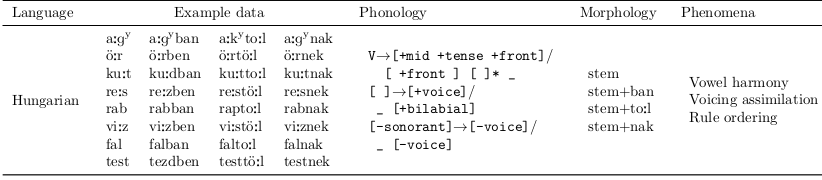
\includegraphics[width=12cm]{exampleProblem4.png}}}\end{textblock*}
\end{frame}

\begin{frame}{What it can do right now}
\tiny  \begin{itemize}
\item \textbf{ Kikurai}: fricatives alternate with stops after nasals
\item \textbf{ Farsi}: Trills alternate with flaps
\item \textbf{ Amharic}: alternation between \textipa{@} \& \textipa{E}
\item \textbf{ Gen}: l/r alternation
\item \textbf{ Greek}: Velar stops alternate with palletized versions before front vowels
  \item \textbf{ Osage}: coronal stops become dentals before central vowels
\item \textbf{ Kishambaa}: voiced/unvoiced nasals alternate
\item \textbf{  Thai}: stops are unreleased word finally
\item \textbf{ Palauan}: a word initial neutralizing rule
\item \textbf{ Quechua}: Velar becomes uvular when followed by uvular (spreading)
\item \textbf{ Lhasa Tibetan}: no contrast between velar/uvular, or voiced/voiceless stops or fricatives
\item \textbf{ Axininca Campa}: stops become glides
\item \textbf{ Kikuyu}: infinitive prefix can surface as either k or \textipa{G}
\item \textbf{ Korean}: vowel harmony, aspiration only surfaces in certain contexts
\item \textbf{ Hungarian}: vowel harmony and voicing assimilation
\item \textbf{ Kikuria}: vowel harmony
\item \textbf{ Farsi}: a deletion rule explains singular/plural
\item \textbf{ Tibetan}: initial consonant cluster reduction explains counting system
\item \textbf{ Makonde}: stress patterns; unstressed vowels are neutralized
\item \textbf{ North Saami}: 3 neutralization rules explain nominative sg essive
\item \textbf{ Samoan}: 2 deletion rules that explain words that sound the same in one inflection being different in another
\item \textbf{     Russian}: devoicing of word final obstruent
\item \textbf{ English}: verbal inflections (voicing assimilation, epenthesis)
\item \textbf{ Finnish}: nominative/partive explained by vowel raising and vowel harmony
\item \textbf{ Kerewe}: Interacting tone rules
\item \textbf{ Polish}: vowel alternations interacting with devoicing of word final obstruent in singular/plural
\item \textbf{ Ancient Greek}: voicing assimilation, deaspiration, deletion rule. Order matters.
\item \textbf{ Serbo-Croatian}: predictable stress, devoicing, neutralizing, epenthesis
\item \textbf{Artificial grammar learning}: Pig Latin, ABB, ABA, AxA, ABx, AAx, Chinese duplication
\end{itemize}

  \begin{textblock*}{5cm}(8.1cm,1cm)
    \Huge
\visible<2->{    Handles 60\% of the textbook}
  \end{textblock*}

  \end{frame}

\begin{frame}[t]{Polish: Final devoicing + Rule ordering}

  \begin{center}
    \begin{tabular}{ll}
      singular&plural\\\hline
      \textipa{dom} & \textipa{domi}\\
      \textipa{kot} & \textipa{koti}\\
      \textipa{lut} & \textipa{lodi}\\
      \textipa{vus} & \textipa{vozi}\\
      \textipa{wuk} & \textipa{wugi}\\
      \textipa{ruk} & \textipa{rogi}\\
      \textipa{bur} & \textipa{bori}\\
      \textipa{\|v{s}um} & \textipa{\|v{s}umi}
    \end{tabular}
  \end{center}

  \pause
  
\vspace{0.5cm}
  
  \textipa{o}$\to$\textipa{u}$/$ \_ [-nasal +voice]\#

  [-sonorant]$\to$[-voice] $/$ \_ \#

  \hline
  
  singular: stem

  plural: stem$ + /\text{i}/$
  

\end{frame}

%% \begin{frame}[t]{Kikuria: vowel harmony}

%%   \begin{center}
%%     \begin{tabular}{ll}
%%      verb&verb for\\\hline
%% \textipa{rema} & \textipa{remera}\\
%% \textipa{roma} & \textipa{romera}\\
%% \textipa{tiga} & \textipa{tegera}\\
%% \textipa{ruga} & \textipa{rogera}\\
%% \textipa{hoora} & \textipa{hoorera}\\
%% \textipa{siika} & \textipa{seekera}\\
%% \textipa{huuta} & \textipa{hootera}\\
%% \textipa{suraaNga} & \textipa{suraaNgera}
%% \end{tabular}
%%   \end{center}

%%     \pause
  
%% \vspace{0.5cm}

%% [+high]$\to$[+middle]$ /$ \_ [-low]* [+middle]

%% \hline
%% verb: stem$ + /\text{a}/$

%% verb for: stem$ + /\text{era}/$

%% \end{frame}

%% \begin{frame}[t]{Makonde: stress patterns}

%%   \begin{center}
%%     \begin{tabular}{lll}
%%       repeated imperative&past&imperative\\\hline
%% \textipa{am\'aNga} & \textipa{am\'ile} & \textipa{\'ama}\\
%% %\textipa{ak\'aNga} & \textipa{ak\'ile} & \textipa{\'aka}\\
%% %\textipa{av\'aNga} & \textipa{av\'ile} & \textipa{\'ova}\\
%% \textipa{am\'aNga} & \textipa{am\'ile} & \textipa{\'oma}\\
%% \textipa{ut\'aNga} & \textipa{ut\'ile} & \textipa{\'uta}\\
%% \textipa{av\'aNga} & \textipa{av\'ile} & \textipa{\'eva}\\
%% \textipa{tav\'aNga} & \textipa{tav\'ile} & \textipa{t\'ava}\\
%% \textipa{uNg\'aNga} & \textipa{uNg\'ile} & \textipa{\'uNga}\\
%% \textipa{pat\'aNga} & \textipa{pat\'ile} & \textipa{p\'ota}
%% \end{tabular}
%%   \end{center}

%%     \pause
  
%% \vspace{0.5cm}


%%   [ ]$\to$[-stress] $/$ \_ [ ]* [ +stress] \\
%%   [+middle -stress]$\to$a $/$ \_ [ ]\\\hline
%% repeated imperative:   stem$ + $\textipa{\'aNga}\\
%% past:  stem$ + $\textipa{\'ile}\\
%% imperative:  stem$ + $\textipa{a}









%% \end{frame}

\begin{frame}{Scaling program synthesis to learn large grammars}
  
  \begin{textblock*}{10cm}(0.5cm,2cm)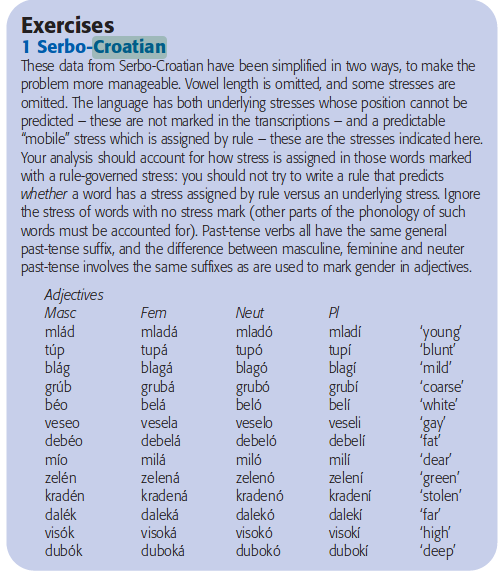
\includegraphics[width=6cm]{Croatian1.png}\end{textblock*}
  \begin{textblock*}{10cm}(6.5cm,2cm)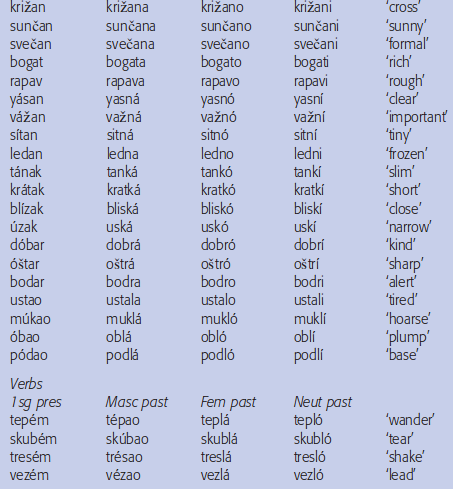
\includegraphics[width=6cm]{Croatian2.png}\end{textblock*}

\end{frame}

%% \begin{frame}{Relaxing the requirement of complete search}

%%   \begin{tikzpicture}
%%     \draw[thick]     (0.1,-0.1) rectangle (4.5,6);
%%     \node at (7.5,3) {$X = \text{observed data}$ };
%%     \node at (2.5,6.25) {Space of all grammars};

    
%%     \node(empty)[align = center] at (0.5,-0.5) {\tiny empty grammar};
%%     \node(emptyp)[fill = cyan,align = center] at (0.5,0.5) {\tiny $\mathcal{G}_0$};    %    \draw[blue,fill = blue] (0.5,0.5) circle (0.1) ;
%%     \draw[thick,->] (empty.north) -- (emptyp.south);

%%     \node(target)[align = center] at (7,5) {\tiny target grammar: best explanation for $X$};
%%     \node(targetGrammar)[green, draw, fill, star, star points=5] at (3.7,5){};%    \draw[yellow,fill = yellow] (2.5,5.5) star (star points = 5);% (0.1) ;
%%     \draw[thick,->] (target.west) -- (targetGrammar.east);

%% \pause
%% \draw[red] (0.5,0.5) circle (2) ;

%% \node at (7.5,2) {\Small $c_1\in X\text{ is a counterexample to }\mathcal{G}_0$};
%% %    };

%%     \pause

%%     \node(g1p)[fill = cyan,align = center] at (1.8,1.8) {\tiny $\mathcal{G}_1$};
%%     \node(g1)[align = center] at (3,-0.5) {\tiny explains $c_1$};  
%%     \draw[thick,->] (g1.north) -- (g1p.south);
%%     \draw[dashed] (emptyp.north) -- (g1p.west);

%%     \pause
%% \draw[red] (g1p.north) circle (2) ;
%% \node at (7.5,1) {\Small $c_2\in X\text{ is a counterexample to }\mathcal{G}_1$};
%% %    };

%%     \pause

%%     \node(g2p)[fill = cyan,align = center] at (3,3.8) {\tiny $\mathcal{G}_2$};
%%     \node(g2)[align = center] at (-0.5,3.9) {\tiny explains $c_2$};  
%%     \draw[thick,->] (g2.east) -- (g2p.west);
%%     \draw[dashed] (g1p.north) -- (g2p.south);

%%     \pause
%%     \draw[dashed] (g2p.north) -- (targetGrammar.south);
%%     \node at (7.5,0) {\Small $c_3\in X\text{ is a counterexample to }\mathcal{G}_2$};
%% \draw[red] (g2p.north) circle (2) ;
%%   \end{tikzpicture}

%% \end{frame}

\begin{frame}{Scaling program synthesis to learn large grammars}
  
  \begin{textblock*}{10cm}(0.5cm,2cm)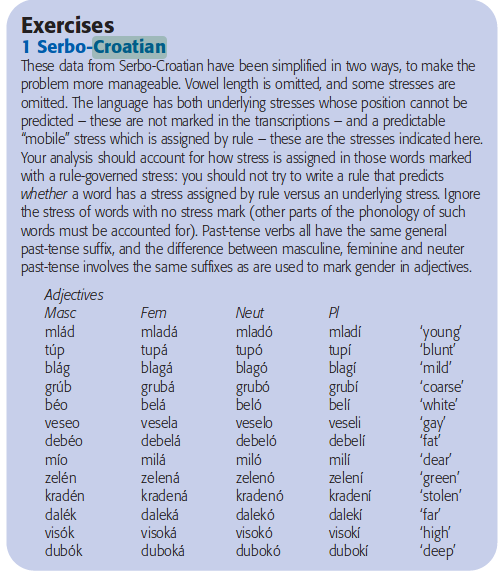
\includegraphics[width=6cm]{Croatian1.png}\end{textblock*}
  \begin{textblock*}{10cm}(6.5cm,2cm)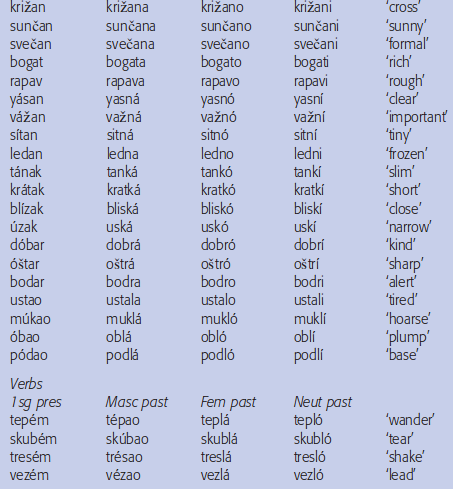
\includegraphics[width=6cm]{Croatian2.png}\end{textblock*}
  
  \begin{textblock*}{10cm}(2cm,3cm)
    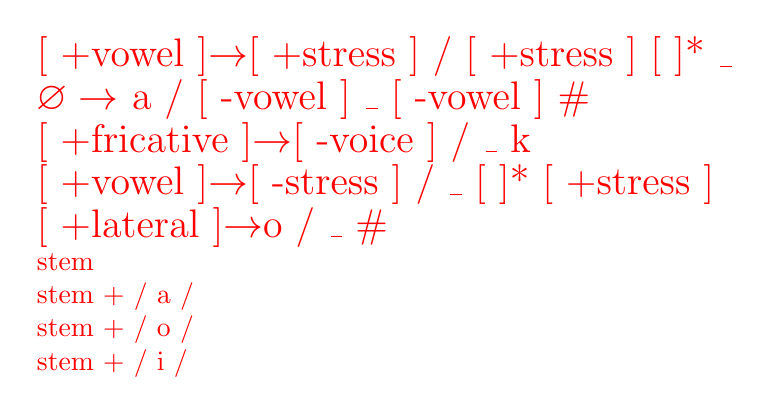
\begin{tikzpicture}
      \node[red,fill = white,align = left]{\Large
        [ +vowel ]$\to$[ +stress ] / [ +stress ] [  ]* \_\\\Large
        $\varnothing\to$ a / [ -vowel ] \_ [ -vowel ] \#\\\Large
        [ +fricative ]$\to$[ -voice ] /  \_ k\\\Large
        [ +vowel ]$\to$[ -stress ] /  \_ [  ]* [ +stress ]\\\Large
        [ +lateral ]$\to$o /  \_ \# \\
        stem \\
       stem + / a /\\
       stem + / o /\\
       stem + / i /
};
      \end{tikzpicture}
\end{textblock*}
\end{frame}

\begin{frame}{}

  \Huge

\Huge  Investigating the inductive bias over grammars

  \end{frame}

\begin{frame}[t]{Motivation: Counting in Tibetan}

    \begin{textblock*}{10cm}(0.5cm,2.5cm)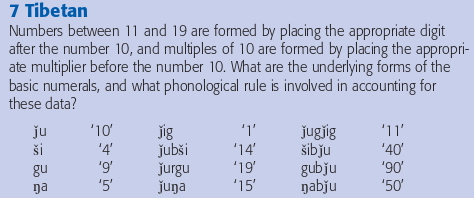
\includegraphics[width=12cm]{Tibetan.png}\end{textblock*}

\end{frame}


\begin{frame}[t]{Motivation: Counting in Tibetan}

  \begin{center}
    \begin{tabular}{l|l}
      Number&Pronunciation\\\hline
      1& \textipa{\v{j}ig}\\
      4& \textipa{\v{s}i}\\
      10&\textipa{\v{j}u}\\
      11&\textipa{\v{j}u+g\v{j}ig} (10+1)\\
      40&\textipa{\v{s}i+b\v{j}u} (4+10)
  \end{tabular}
    \end{center}


%%   \vspace{1cm}

%%   Explanation:

%%   \textipa{\v{j}ig} (``1'') is really     \textipa{g\v{j}ig}

%%   \textipa{\v{j}u} (``10'') is really     \textipa{b\v{j}u}

%%   \begin{textblock*}{10cm}(8.3cm,6.5cm)\includegraphics[width=3cm]{Tim.jpeg}\end{textblock*}

%% \textbf{Program:}

%% C$\to \varnothing $/\# C \_

%% (Delete initial cluster of consonants)
\end{frame}

\begin{frame}[t]{Motivation: Counting in Tibetan}

  \begin{center}
    \begin{tabular}{l|l}
      Number&Pronunciation\\\hline
      1& \textipa{\v{j}ig}\\
      4& \textipa{\v{s}i}\\
      10&\textipa{\v{j}u}\\
      11&\textipa{\v{j}u+g\v{j}ig} (10+1)\\
      40&\textipa{\v{s}i+b\v{j}u} (4+10)
  \end{tabular}
    \end{center}


  \vspace{1cm}

  Explanation:

  \textipa{\v{j}ig} (``1'') is really     \textipa{g\v{j}ig}

  \textipa{\v{j}u} (``10'') is really     \textipa{b\v{j}u}

%  \begin{textblock*}{10cm}(8.3cm,6.5cm)\includegraphics[width=3cm]{Tim.jpeg}\end{textblock*}

\textbf{Program:}

C$\to \varnothing $/\# \_ C

(Delete initial cluster of consonants)
\end{frame}

\begin{frame}[t]{Counting in Tibetan}

  \begin{center}
    \begin{tabular}{l|l}
      Number&Pronunciation\\\hline
      1& \textipa{\v{j}ig}\\
      4& \textipa{\v{s}i}\\
      10&\textipa{\v{j}u}\\
      11&\textipa{\v{j}u+g\v{j}ig} (10+1)\\
      40&\textipa{\v{s}i+b\v{j}u} (4+10)
  \end{tabular}
    \end{center}


  \vspace{1cm}

  Explanation:

  \textipa{\v{j}ig} (``1'') is really     \textipa{g\v{j}ig}

  \textipa{\v{j}u} (``10'') is really     \textipa{b\v{j}u}

\textbf{Program:}

[-nasal]$\to \varnothing $/\# \_

\textbf{Delete initial nonnasal???}
\end{frame}

\begin{frame}{}
  \large

%  \centering

  \textbf{Problem:} \\Probable grammar $\not=$ grammars children/linguists prefer

  \pause

  \\\\\vspace{1cm}

  \textbf{Solution:}\\ Get a better inductive bias (a better universal grammar)

  \end{frame}

%% \begin{frame}{Learning which features are important}

%% \centering  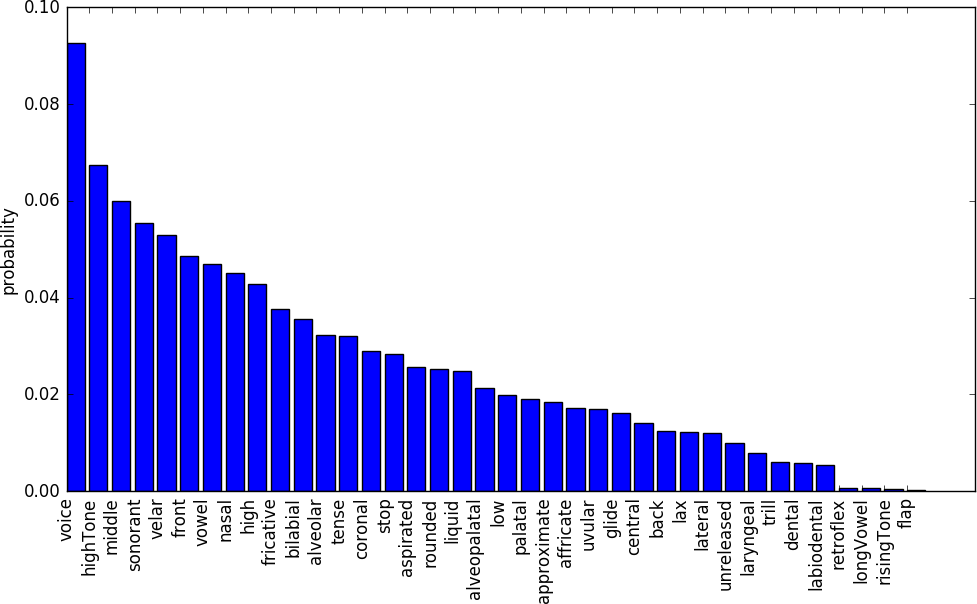
\includegraphics[width = 11.5cm]{featureFrequencies.png}

%% \end{frame}

\begin{frame}{Learning what rules look like}

\centering  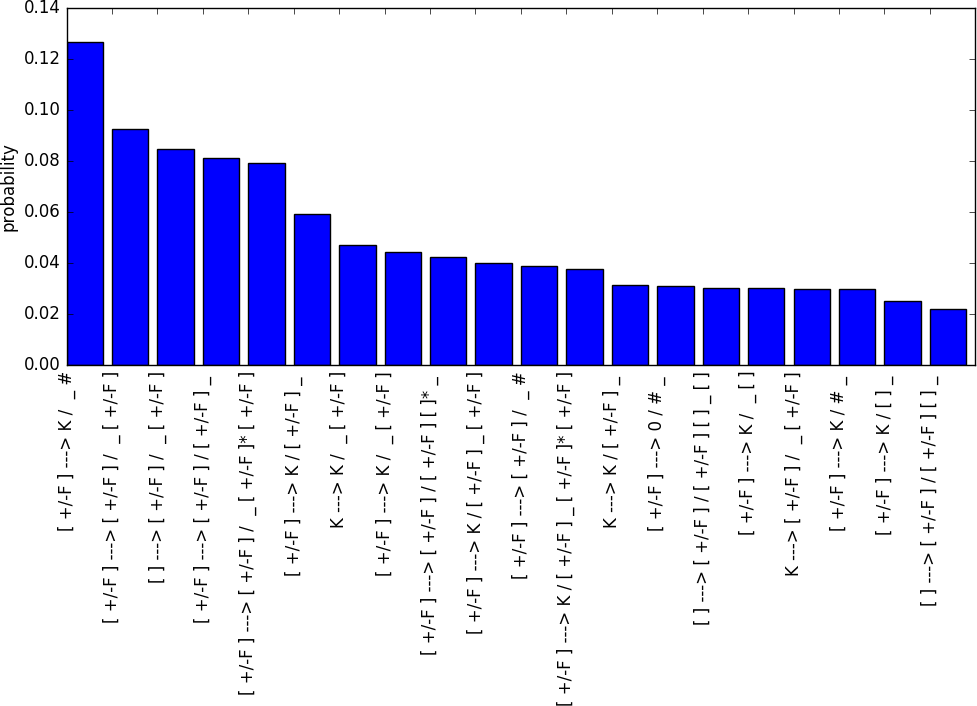
\includegraphics[width = 11.5cm]{skeletonFrequencies.png}

\end{frame}

\begin{frame}{Learning a (fragment) grammar over grammars}
  Fragment grammars: O'Donnell 2011
  \small
\begin{tabular}{ll}
    FEATUREMATRIX $\to$& [ -voice ]\\
     FEATUREMATRIX $\to$& [ -sonorant ]\\
 FEATUREMATRIX $\to$& [ +voice ]\\
 FEATUREMATRIX $\to$& [ +tense ]\\
 FEATUREMATRIX $\to$& [ +highTone ]\\
 FEATUREMATRIX $\to$& [ +middle ]\\
 TRIGGER $\to$& [ +sibilant ]\\
 TRIGGER $\to$& [ ] [ +highTone ]\\
 TRIGGER $\to$& [ +stop +voice ]\\
 TRIGGER $\to$& [ -low ]\\
 TRIGGER $\to$& [ ]* FEATUREMATRIX\\
 RULE $\to$& [ -vowel ] $\to$ $\varnothing$ / TRIGGER \_ TRIGGER\\
 RULE $\to$& [ +low ] $\to$ CONSTANT / [ ]* FEATUREMATRIX \_\\
 RULE $\to$& [ ] $\to$ [ +voice ] / \_ TRIGGER\\
 RULE $\to$& CONSTANT $\to$ CONSTANT / [ ] \_ TRIGGER\\
 RULE $\to$& [ ] $\to$ [ -highTone ] / TRIGGER \_ TRIGGER\\
 RULE $\to$& [ -sonorant ] $\to$ [ -voice ] / \_ \#\\
 RULE $\to$& [ ] $\to$ FC / TRIGGER \_ [ ] FEATUREMATRIX\\
    \end{tabular}
\end{frame}
\begin{frame}{Learning a (fragment) grammar over grammars}
  Fragment grammars: O'Donnell 2011
  \small
  \begin{tabular}{ll}
    FEATUREMATRIX $\to$& [ -voice ]\\
     FEATUREMATRIX $\to$& [ -sonorant ]\\
 FEATUREMATRIX $\to$& [ +voice ]\\
 FEATUREMATRIX $\to$& [ +tense ]\\
 FEATUREMATRIX $\to$& [ +highTone ]\\
 FEATUREMATRIX $\to$& [ +middle ]\\
 TRIGGER $\to$& [ +sibilant ]\\
 TRIGGER $\to$& [ ] [ +highTone ]\\
 TRIGGER $\to$& [ +stop +voice ]\\
 TRIGGER $\to$& [ -low ]\\
 TRIGGER $\to$& [ ]* FEATUREMATRIX\\
 RULE $\to$& {\color{red}[ -vowel ] $\to$ $\varnothing$ / TRIGGER \_ TRIGGER}\\
 RULE $\to$& [ +low ] $\to$ CONSTANT / [ ]* FEATUREMATRIX \_\\
 RULE $\to$& [ ] $\to$ [ +voice ] / \_ TRIGGER\\
 RULE $\to$& CONSTANT $\to$ CONSTANT / [ ] \_ TRIGGER\\
 RULE $\to$& [ ] $\to$ [ -highTone ] / TRIGGER \_ TRIGGER\\
 RULE $\to$& {\color{red}[ -sonorant ] $\to$ [ -voice ] / \_ \#}\\
 RULE $\to$& [ ] $\to$ FC / TRIGGER \_ [ ] FEATUREMATRIX\\
  \end{tabular}

    
\end{frame}

\begin{frame}{Learning a (fragment) grammar over grammars}
  Fragment grammars: O'Donnell 2011
  \small
  \begin{tabular}{ll}
    FEATUREMATRIX $\to$& [ -voice ]\\
     FEATUREMATRIX $\to$& [ -sonorant ]\\
 FEATUREMATRIX $\to$& [ +voice ]\\
 FEATUREMATRIX $\to$& [ +tense ]\\
 FEATUREMATRIX $\to$& [ +highTone ]\\
 FEATUREMATRIX $\to$& [ +middle ]\\
 TRIGGER $\to$& [ +sibilant ]\\
 TRIGGER $\to$& [ ] [ +highTone ]\\
 TRIGGER $\to$& [ +stop +voice ]\\
 TRIGGER $\to$& [ -low ]\\
 TRIGGER $\to$& [ ]* FEATUREMATRIX\\
 RULE $\to$& {\color{red}[ -vowel ] $\to$ $\varnothing$ / TRIGGER \_ TRIGGER}\\
 RULE $\to$& [ +low ] $\to$ CONSTANT / [ ]* FEATUREMATRIX \_\\
 RULE $\to$& [ ] $\to$ [ +voice ] / \_ TRIGGER\\
 RULE $\to$& CONSTANT $\to$ CONSTANT / [ ] \_ TRIGGER\\
 RULE $\to$& [ ] $\to$ [ -highTone ] / TRIGGER \_ TRIGGER\\
 RULE $\to$& {\color{red}[ -sonorant ] $\to$ [ -voice ] / \_ \#}\\
 RULE $\to$& [ ] $\to$ FC / TRIGGER \_ [ ] FEATUREMATRIX\\
  \end{tabular}

    \begin{textblock*}{6cm}(3cm,2.5cm)
         \textblockcolor{lightgray}
         \hspace{0.7cm}  \large    In light of this UG, the \\
         \hspace{0.7cm}system revises its rule for \\
         \hspace{0.7cm}Tibetan to match the good \\
         \hspace{0.7cm}linguistics students judgment:\\
{\color{red}\hspace{0.3}[ -vowel ] $\to$ $\varnothing$ / } \# \_ [-vowel]
    \end{textblock*}
\end{frame}

\begin{frame}{}

  \Huge
  Problems with minimum description length

  \end{frame}

\begin{frame}{Problems with compression}
  \begin{tabular}{ll}
\textipa{varit} & \textipa{varihin}\\
\textipa{oahpis} & \textipa{oahpisin}\\
\textipa{bissobeahtset} & \textipa{bissobeahtsehin}\\
\textipa{yaaPmin} & \textipa{yaaPmimin}\\
\textipa{gahpir} & \textipa{gahpirin}\\
\textipa{gaauhtsis} & \textipa{gaauhtsisin}\\
\textipa{be\v{s}tor} & \textipa{be\v{s}torin}\\
\textipa{heevemeahhtun} & \textipa{heevemeahhtunin}\\
\textipa{bissomeahtun} & \textipa{bissomeahtumin}\\
\textipa{laDas} & \textipa{laDasin}\\
\textipa{heaNkkan} & \textipa{heaNkkanin}\\
\textipa{yaman} & \textipa{yamanin}
\end{tabular}

\end{frame}

\begin{frame}{Problems with compression}
  \begin{tabular}{ll}
\textipa{varit} & \textipa{varihin}\\
\textipa{oahpis} & \textipa{oahpisin}\\
\textipa{bissobeahtset} & \textipa{bissobeahtsehin}\\
{\color{red}\textipa{yaaPmin}} & {\color{red}\textipa{yaaPmimin}}\\
\textipa{gahpir} & \textipa{gahpirin}\\
\textipa{gaauhtsis} & \textipa{gaauhtsisin}\\
\textipa{be\v{s}tor} & \textipa{be\v{s}torin}\\
{\color{red}\textipa{heevemeahhtun}} &{\color{red} \textipa{heevemeahhtunin}}\\
{\color{red}\textipa{bissomeahtun}} &{\color{red} \textipa{bissomeahtumin}}\\
\textipa{laDas} & \textipa{laDasin}\\
{\color{red}\textipa{heaNkkan}} &{\color{red} \textipa{heaNkkanin}}\\
{\color{red}\textipa{yaman}} &{\color{red} \textipa{yamanin}}
  \end{tabular}

  \visible<2->{
    \begin{textblock*}{5cm}(7cm,1.5cm)
               \textblockcolor{white}
      \Large
      \begin{tabular}{l}
        \texttt{stem}$ + $/in/\\
        m$\to$n word finally\\\\
        \textipa{yaaPmim}$\to$\textipa{yaaPmin}\\
        \textipa{yaaPmim}$+$\textipa{in}$\to$\textipa{yaaPmimin}
        \end{tabular}
  \end{textblock*}}

\end{frame}

\begin{frame}{Problems with compression}
  \begin{tabular}{ll}
\textipa{varit} & \textipa{varihin}\\
\textipa{oahpis} & \textipa{oahpisin}\\
\textipa{bissobeahtset} & \textipa{bissobeahtsehin}\\
{\color{red}\textipa{yaaPmin}} & {\color{red}\textipa{yaaPmimin}}\\
\textipa{gahpir} & \textipa{gahpirin}\\
\textipa{gaauhtsis} & \textipa{gaauhtsisin}\\
\textipa{be\v{s}tor} & \textipa{be\v{s}torin}\\
{\color{red}\textipa{heevemeahhtun}} &{\color{red} \textipa{heevemeahhtunin}}\\
{\color{red}\textipa{bissomeahtun}} &{\color{red} \textipa{bissomeahtumin}}\\
\textipa{laDas} & \textipa{laDasin}\\
{\color{red}\textipa{heaNkkan}} &{\color{red} \textipa{heaNkkanin}}\\
{\color{red}\textipa{yaman}} &{\color{red} \textipa{yamanin}}
  \end{tabular}

  \begin{textblock*}{5cm}(7cm,1.5cm)\textblockcolor{white}
      \Large
      \begin{tabular}{l}
        \texttt{stem}$ + $/i{\color{red}m}/\\
        m$\to$n word finally\\\\
        \textipa{yaaPmim}$\to$\textipa{yaaPmin}\\
        \textipa{yaaPmim}$+$i{\color{red}m}$\to$\\\textipa{yaaPmimim}$\to$\\\textipa{yaaPmimin}
      \end{tabular}
      \visible<2->{\Huge MDL unchanged!}
      
  \end{textblock*}
      \visible<3->{\vspace{1cm}\color{red} $    \text{cost}(\text{model}; \text{data}) = \text{cost}(\text{model}) + \sum_{x\in \text{data}}\text{cost}(x ; \text{model}) + \text{runtimeCost}(x ; \text{model})$}
\end{frame}


\begin{frame}{Contributions}

  Engineered new approaches to grammar learning drawn from program synthesis. Allows exact study of simplicity trade-offs between different grammars.

  \vspace{1cm}
  
  A system that can learn many morphophonologies, both natural and artificial, from relatively small amounts of data

  \vspace{1cm}
  
  Learning to learn phonological rules as a way of estimating and probing universal grammar

  \pause

  \vspace{1cm}
  

  \textbf{The end.}
  
\end{frame}


\end{document}
